\documentclass[11pt,a4paper]{report}
% ============================================================
%  Shared preamble: colours, typography, boxes, tables, UML/TikZ styles
% ============================================================
\usepackage[T1]{fontenc}
\usepackage[utf8]{inputenc}
\usepackage{mathpazo}
\usepackage[scaled=0.92]{helvet}
\usepackage[a4paper,margin=2.4cm,headheight=15pt]{geometry}
\usepackage[table,dvipsnames]{xcolor}
\usepackage{microtype}
\usepackage{amsmath}
\usepackage{graphicx}
\usepackage{array,booktabs,longtable,tabularx,multirow}
\usepackage{enumitem}
\usepackage{float}
\usepackage[font=small,labelfont={bf,color=navy},textfont=it,skip=6pt]{caption}
\usepackage{fancyhdr}
\usepackage{titlesec}
\usepackage{listings}
\usepackage{tikz}
\usetikzlibrary{arrows.meta,positioning,shapes.geometric,shapes.multipart,shapes.misc,fit,backgrounds,calc,decorations.pathreplacing,patterns}
\usepackage{pgfgantt}
\usepackage[most]{tcolorbox}
\usepackage[colorlinks=true,linkcolor=teal,urlcolor=teal,citecolor=teal]{hyperref}

% ---------- Colour palette ----------
\definecolor{navy}{HTML}{0B2545}
\definecolor{teal}{HTML}{0E8F9C}
\definecolor{tealdark}{HTML}{0A6B75}
\definecolor{amber}{HTML}{F2A33A}
\definecolor{coral}{HTML}{D9534F}
\definecolor{violet}{HTML}{6C4FA1}
\definecolor{leaf}{HTML}{3E9B5F}
\definecolor{mist}{HTML}{EEF3F8}
\definecolor{mint}{HTML}{DDF3F1}
\definecolor{sand}{HTML}{FDF1DC}
\definecolor{blush}{HTML}{FBE3E1}
\definecolor{lilac}{HTML}{E9E3F5}
\definecolor{slate}{HTML}{4A5568}
\definecolor{rowgray}{HTML}{F3F6FA}

% ---------- Project macros (change here only) ----------
\newcommand{\projname}{DocuMind AI}
\newcommand{\projfull}{Intelligent Document Processing and Automated ERP Ingestion System}
\newcommand{\studentname}{Tuheu Tchoubi Pempeme Moussa Fahdil}
\newcommand{\supervisorname}{[Supervisor name -- to be completed]}
\newcommand{\docversion}{2.0}
\newcommand{\docdate}{October 2026}

% ---------- Headings ----------
\titleformat{\chapter}[display]
  {\sffamily\bfseries\color{navy}}
  {\vspace*{-0.5cm}\color{teal}\fontsize{54}{54}\selectfont\thechapter}
  {0.2cm}
  {\Huge}
  [\vspace{2pt}{\color{teal}\titlerule[2.2pt]}]
\titlespacing*{\chapter}{0pt}{0pt}{26pt}
\titleformat{\section}{\sffamily\Large\bfseries\color{navy}}{\color{teal}\thesection}{0.6em}{}
\titleformat{\subsection}{\sffamily\large\bfseries\color{tealdark}}{\thesubsection}{0.6em}{}
\titleformat{\subsubsection}{\sffamily\normalsize\bfseries\color{slate}}{\thesubsubsection}{0.6em}{}
\titlespacing*{\section}{0pt}{16pt}{6pt}
\titlespacing*{\subsection}{0pt}{12pt}{4pt}

% ---------- Header / footer ----------
\pagestyle{fancy}
\fancyhf{}
\renewcommand{\headrulewidth}{0.6pt}
\renewcommand{\headrule}{\hbox to\headwidth{\color{teal}\leaders\hrule height \headrulewidth\hfill}}
\renewcommand{\footrulewidth}{0pt}
\fancyhead[L]{\small\sffamily\color{navy}\projname}
\fancyhead[R]{\small\sffamily\color{slate}\nouppercase{\leftmark}}
\fancyfoot[C]{\small\sffamily\color{slate}\thepage}
\fancypagestyle{plain}{\fancyhf{}\fancyfoot[C]{\small\sffamily\color{slate}\thepage}\renewcommand{\headrulewidth}{0pt}}

% ---------- Lists, spacing ----------
\setlist{itemsep=2pt,topsep=4pt,parsep=0pt}
\setlist[itemize]{label=\textcolor{teal}{\textbullet}}
\setlist[enumerate]{label=\textcolor{teal}{\bfseries\arabic*.}}
\setlength{\parindent}{0pt}
\setlength{\parskip}{6pt}
\renewcommand{\arraystretch}{1.25}
\setcounter{tocdepth}{2}

% ---------- Call-out boxes ----------
\tcbset{calloutbase/.style={enhanced,breakable,sharp corners,boxrule=0pt,leftrule=3.5pt,
  left=8pt,right=8pt,top=6pt,bottom=6pt,fonttitle=\sffamily\bfseries,coltitle=navy,
  attach boxed title to top left={yshift=-2mm},
  boxed title style={colback=white,boxrule=0pt,top=0pt,bottom=0pt,left=0pt}}}
\newtcolorbox{infobox}[1][Note]{calloutbase,colback=mint,colframe=teal,title={#1}}
\newtcolorbox{warnbox}[1][Important]{calloutbase,colback=sand,colframe=amber,title={#1}}
\newtcolorbox{statusbox}[1][Status]{calloutbase,colback=lilac,colframe=violet,title={#1}}
\newtcolorbox{goalbox}[1][Goal]{calloutbase,colback=mist,colframe=navy,title={#1}}

% ---------- Tables ----------
\newcolumntype{L}[1]{>{\raggedright\arraybackslash}p{#1}}
\newcolumntype{C}[1]{>{\centering\arraybackslash}p{#1}}
\newcommand{\hdr}[1]{\textcolor{white}{\sffamily\bfseries #1}}
\newcommand{\tblstart}{\rowcolors{2}{white}{rowgray}\arrayrulecolor{teal!60}}
\newcommand{\hdrrow}{\rowcolor{navy}}
\newcommand{\must}{\textcolor{coral}{\sffamily\bfseries Must}}
\newcommand{\should}{\textcolor{amber!85!black}{\sffamily\bfseries Should}}
\newcommand{\could}{\textcolor{tealdark}{\sffamily\bfseries Could}}
\newcommand{\wont}{\textcolor{slate}{\sffamily\bfseries Won't (now)}}
\newcommand{\done}{\textcolor{leaf}{\sffamily\bfseries Done}}
\newcommand{\inprog}{\textcolor{amber!85!black}{\sffamily\bfseries Partial}}
\newcommand{\todo}{\textcolor{slate}{\sffamily\bfseries Planned}}
\newcommand{\code}[1]{\texttt{\small #1}}

% ---------- Code listings ----------
\lstdefinestyle{docu}{basicstyle=\ttfamily\footnotesize,backgroundcolor=\color{mist},
  frame=l,rulecolor=\color{teal},framerule=3pt,xleftmargin=10pt,framexleftmargin=6pt,
  keywordstyle=\color{tealdark}\bfseries,commentstyle=\color{slate}\itshape,
  stringstyle=\color{violet},showstringspaces=false,breaklines=true,columns=fullflexible,
  aboveskip=8pt,belowskip=8pt}
\lstset{style=docu}

% ---------- TikZ / UML styles ----------
\tikzset{
  every picture/.append style={font=\sffamily\small},
  box/.style={rectangle,rounded corners=3pt,draw=navy,line width=0.7pt,fill=mist,align=center,
              minimum height=0.8cm,inner sep=4pt},
  boxT/.style={box,fill=mint,draw=tealdark},
  boxA/.style={box,fill=sand,draw=amber!80!black},
  boxV/.style={box,fill=lilac,draw=violet},
  boxC/.style={box,fill=blush,draw=coral},
  boxN/.style={box,fill=navy,draw=navy,text=white},
  arr/.style={-{Stealth[length=2.6mm,width=1.9mm]},line width=0.7pt,color=navy},
  arrd/.style={-{Stealth[length=2.6mm,width=1.9mm]},line width=0.7pt,color=slate,dashed},
  lbl/.style={font=\sffamily\scriptsize,color=slate,fill=white,inner sep=1.2pt},
  state/.style={rectangle,rounded corners=8pt,draw=tealdark,fill=mint,line width=0.8pt,
                minimum width=2.5cm,minimum height=0.9cm,align=center,font=\sffamily\footnotesize\bfseries},
  stateA/.style={state,fill=sand,draw=amber!80!black},
  stateC/.style={state,fill=blush,draw=coral},
  stateV/.style={state,fill=lilac,draw=violet},
  initial/.style={circle,fill=navy,minimum size=0.35cm,inner sep=0pt},
  final/.style={circle,draw=navy,line width=0.9pt,minimum size=0.5cm,inner sep=0pt,
                path picture={\fill[navy] (path picture bounding box.center) circle (0.17cm);}},
  uclass/.style={rectangle split,rectangle split parts=3,draw=navy,line width=0.8pt,fill=white,
                 font=\sffamily\scriptsize,text width=3.55cm,inner sep=3pt,align=left,
                 rectangle split part fill={mint,white,white}},
  uclass2/.style={rectangle split,rectangle split parts=2,draw=navy,line width=0.8pt,fill=white,
                 font=\sffamily\scriptsize,text width=3.55cm,inner sep=3pt,align=left,
                 rectangle split part fill={mint,white}},
  uiface/.style={uclass2,rectangle split part fill={sand,white}},
  uenum/.style={uclass2,rectangle split part fill={lilac,white}},
  ucase/.style={ellipse,draw=tealdark,fill=mint,line width=0.7pt,align=center,
                font=\sffamily\scriptsize,minimum height=0.8cm,inner xsep=3pt},
  lifeline/.style={dashed,color=slate,line width=0.6pt},
  msg/.style={-{Stealth[length=2.4mm,width=1.7mm]},line width=0.65pt,color=navy},
  ret/.style={-{Stealth[length=2.4mm,width=1.7mm]},line width=0.65pt,color=slate,dashed},
}
% stick-figure actor: \actor{name}{x}{y}{label}
\newcommand{\actor}[4]{%
  \begin{scope}[shift={(#2,#3)},color=navy,line width=0.9pt]
    \draw[fill=sand] (0,0.95) circle (0.2);
    \draw (0,0.75)--(0,0.1) (-0.35,0.55)--(0.35,0.55) (0,0.1)--(-0.28,-0.4) (0,0.1)--(0.28,-0.4);
    \node[font=\sffamily\scriptsize\bfseries,text=navy,align=center,below] (#1) at (0,-0.38) {#4};
  \end{scope}}
% class-name helper (centred bold)
\newcommand{\cname}[1]{\centerline{\bfseries #1}}
\newcommand{\stereo}[1]{\guillemotleft\,#1\,\guillemotright}

\hypersetup{pdftitle={DocuMind AI - Project Design Document},pdfauthor={Tuheu Tchoubi Pempeme Moussa Fahdil}}
\begin{document}
\begin{titlepage}
\newgeometry{margin=0cm}
\thispagestyle{empty}
\begin{tikzpicture}[remember picture,overlay]
  \fill[navy] (current page.north west) rectangle ([yshift=-17.5cm]current page.north east);
  \fill[teal] ([yshift=-17.5cm]current page.north west) rectangle ([yshift=-17.9cm]current page.north east);
  \fill[amber] ([yshift=-17.9cm]current page.north west) rectangle ([yshift=-18.1cm]current page.north east);
  % decorative document / network motif
  \begin{scope}[shift={([xshift=-8.2cm,yshift=-4.6cm]current page.north east)},opacity=0.9]
    \draw[teal!70,line width=1pt,fill=white!8!navy] (0,0) rectangle (2.6,3.4);
    \foreach \y in {0.5,0.9,1.3,1.7,2.1} {\draw[teal!70,line width=0.8pt] (0.3,\y) -- (2.3,\y);}
    \draw[amber,line width=1.4pt,fill=amber!25!navy] (0.3,2.5) rectangle (1.5,2.9);
    \draw[-{Stealth},amber,line width=1.2pt] (2.8,1.7) -- (4.0,1.7);
    \draw[teal!70,line width=1pt,fill=white!8!navy] (4.2,0.9) rectangle (5.3,2.5);
    \foreach \y in {1.2,1.6,2.0} {\draw[teal!70,line width=0.8pt] (4.4,\y) -- (5.1,\y);}
  \end{scope}
  \node[anchor=west,text=white,font=\sffamily\bfseries\fontsize{40}{44}\selectfont] at ([xshift=2.4cm,yshift=-9.3cm]current page.north west) {\projname};
  \node[anchor=west,text=teal!30,font=\sffamily\fontsize{15}{19}\selectfont,text width=15cm] at ([xshift=2.4cm,yshift=-11.5cm]current page.north west) {Intelligent Document Processing and\\ Automated ERP Ingestion System};
  \node[anchor=west,text=white,font=\sffamily\small,text width=15cm] at ([xshift=2.4cm,yshift=-13.7cm]current page.north west) {Project Requirements, Architecture, UML Models and Implementation Plan};
  \node[anchor=west,text=amber,font=\sffamily\bfseries\footnotesize] at ([xshift=2.4cm,yshift=-15.3cm]current page.north west) {OCR \ $\cdot$ \ INFORMATION EXTRACTION \ $\cdot$ \ VALIDATION \ $\cdot$ \ ERP AUTOMATION};
  \node[anchor=west,text=white!70,font=\sffamily\scriptsize] at ([xshift=2.4cm,yshift=-3.0cm]current page.north west) {ICT UNIVERSITY \ $\cdot$ \ FACULTY OF ICT \ $\cdot$ \ DEPARTMENT OF COMPUTER SCIENCE};
\end{tikzpicture}
\begin{tikzpicture}[remember picture,overlay]
\node[anchor=north west,text width=15.5cm,font=\sffamily\small] at ([xshift=2.4cm,yshift=-19.3cm]current page.north west) {%
\begin{tabular}{@{}L{3.2cm}L{11cm}@{}}
\textcolor{teal}{\bfseries Student}   & \studentname\\
\textcolor{teal}{\bfseries Programme} & B.Sc. Computer Science, final-year project\\
\textcolor{teal}{\bfseries Supervisor}& \supervisorname\\
\textcolor{teal}{\bfseries Institution}& The ICT University, Cameroon\\
\textcolor{teal}{\bfseries Version}    & \docversion \ -- \docdate\\
\end{tabular}};
\end{tikzpicture}
\restoregeometry
\end{titlepage}

\pagenumbering{roman}
\chapter*{Document Control}
\addcontentsline{toc}{chapter}{Document Control}
\tblstart\small
\begin{longtable}{L{3.4cm}L{11.0cm}}
\hdrrow \hdr{Item} & \hdr{Description}\\ \endhead
Purpose & Define the problem, scope, requirements, system design, UML models, data model, security, testing and implementation plan for \projname.\\
Intended readers & Student developer, academic supervisor, evaluators and future maintainers.\\
Version & \docversion{} (\docdate). Supersedes version 1.0, which used a 12-step roadmap and unlabelled diagrams.\\
Status & Design specification plus an honest implementation-status chapter (Chapter~\ref{ch:status}). Performance targets are provisional until measured.\\
Working name & \projname{} is a \emph{proposed} name. Check availability before any commercial use.\\
Companion document & \emph{Phase 1 -- Requirements Analysis and Planning} (separate file) contains the complete Phase 1 deliverable.\\
Primary technologies & Python, FastAPI, MySQL, Flutter Web, OpenCV, PyTorch, Docker; Kubernetes in a later stage.\\
Important limitation & No OCR accuracy, ERP compatibility or performance result is claimed here. Such results must come from experiments.\\
\hline
\end{longtable}

\begin{statusbox}[What changed in version 2.0]
\begin{itemize}
\item New colour theme and a consistent set of UML-style diagrams, drawn as editable TikZ code.
\item The roadmap now follows the 18-phase plan; the prototype is limited to \textbf{invoices}.
\item Requirements were extended (FR-21, FR-22) and linked to provisional success metrics.
\item A new chapter records what is implemented, what is only written, and what is still planned.
\end{itemize}
\end{statusbox}
\clearpage

\chapter*{Abstract}
\addcontentsline{toc}{chapter}{Abstract}
Organisations receive invoices and other business documents as paper scans, PDFs and images. Manual data entry is slow, repetitive and prone to transcription errors. This project proposes \projname, an Intelligent Document Processing (IDP) and automated ERP ingestion system that accepts a document, improves its image quality, recognises its text, extracts structured fields, validates them, routes uncertain cases to a human reviewer and prepares approved records for an Enterprise Resource Planning (ERP) system.

The solution combines a trainable optical character recognition (OCR) component with explicit extraction and validation rules. Image preprocessing uses OpenCV; text recognition is developed with PyTorch using a CRNN network trained with Connectionist Temporal Classification (CTC) loss. French and English are the target languages, and the first prototype is limited to invoices. An established OCR engine serves as a baseline so that the custom model can be evaluated honestly. The backend uses FastAPI and MySQL; a Flutter Web dashboard supports upload, review and monitoring. The system starts as a modular monolith, is containerised with Docker, and is separated into services and deployed on Kubernetes only after the interfaces are stable.

This document specifies requirements, architecture, UML models, data design, security, testing and a phased plan. Measured results will replace the provisional targets once experiments have been run.

\medskip\noindent\textbf{Keywords:} intelligent document processing, OCR, information extraction, human-in-the-loop, ERP integration, FastAPI, Flutter, MySQL, PyTorch.
\clearpage
\tableofcontents
\clearpage
\listoffigures
\clearpage
\listoftables
\clearpage
\pagenumbering{arabic}
\setcounter{page}{1}

\chapter{Introduction}
\section{Background}
Business and public-sector workflows depend on information received in semi-structured or unstructured documents. A clerk opens a PDF, finds the supplier name, invoice number, date, tax amount and total, and types them into a business application. Repeated across hundreds of documents, this consumes staff time and introduces errors.

OCR converts visual text into machine-readable text, but OCR alone does not solve the problem. A practical system must also locate the relevant fields, normalise values, apply business rules, preserve the source document, track corrections and deliver approved data to the target system.

\section{Problem Statement}
There is a gap between incoming digital documents and structured business records. A basic OCR tool returns text without knowing which text is the invoice number, or whether the total agrees with the subtotal and tax. A useful pipeline must connect acquisition, recognition, extraction, validation, human review and controlled ERP delivery in a traceable workflow.

\section{Aim}
To design and implement a secure, modular document-processing system that extracts structured information from French and English invoices and prepares validated records for ERP ingestion.

\section{Specific Objectives}
\begin{enumerate}
\item Provide secure document upload and lifecycle tracking.
\item Preprocess scanned images to improve text readability.
\item Develop and evaluate a trainable OCR model for French and English text.
\item Extract key invoice fields using configurable rules and layout information.
\item Compute field-level confidence and identify records that need human review.
\item Validate fields using format checks, required-field checks, duplicate detection and arithmetic rules.
\item Provide a dashboard to review, correct, approve, reject and track documents.
\item Store metadata, extracted values, validation outcomes and audit events in MySQL.
\item Expose controlled interfaces to an ERP adapter or a sandbox ERP endpoint.
\item Package the system with Docker and document a Kubernetes path.
\end{enumerate}

\section{Research and Engineering Questions}
\begin{itemize}
\item How much does image preprocessing improve recognition on the selected dataset?
\item How does the custom OCR model compare with an established baseline engine?
\item Which combination of confidence, validation rules and human review balances automation and correctness?
\item How can documents be processed reliably without losing traceability?
\item How can ERP-specific code be isolated from document-processing logic?
\end{itemize}

\section{Expected Contribution}
The contribution is an integrated, measurable prototype, not an unsupported claim that a custom OCR model beats existing tools. The work combines a trainable recogniser, domain-specific extraction and validation, human review, auditability and a replaceable ERP adapter. The comparison experiment will show where the custom component works well and where it needs improvement.

\begin{infobox}[Project name]
The working name \projname{} comes from the naming shortlist in the planning phase. It is a suggestion, not a verified trademark or domain. The name is defined in one place (\texttt{\textbackslash projname}) so it can be changed everywhere at once.
\end{infobox}

\chapter{Scope, Users and Assumptions}
\section{Initial Scope}
The first version handles \textbf{invoices} only (supplier invoices received as PDF, PNG or JPEG), in French and English. Purchase orders, receipts, forms and administrative requests are extensions for later versions. The ERP stage uses a sandbox API or a clearly labelled mock adapter until the target ERP and its interface are confirmed.

\section{Out of Scope for the First Prototype}
\begin{itemize}
\item Fully autonomous posting of every document without human review.
\item Support for every document type, language, handwriting style or layout.
\item A production connection to an ERP whose API, schema and authentication are not yet known.
\item Claims of legal or accounting compliance without review against applicable rules.
\item Kubernetes operations before the containerised application is stable and tested.
\end{itemize}

\section{Stakeholders and Roles}
{\tblstart\small
\begin{longtable}{L{3.0cm}L{4.4cm}L{6.6cm}}
\hdrrow \hdr{Role} & \hdr{Responsibility} & \hdr{Permissions / use}\\ \endhead
Administrator & Manage users, configuration, thresholds and integration settings. & Create or deactivate users, assign roles, view system status, configure rules.\\
Document operator & Upload and monitor incoming documents. & Upload, view status of permitted records.\\
Reviewer / accountant & Check extracted fields and resolve uncertainty. & Correct fields, add notes, approve or reject records.\\
Integration service account & Transfer approved records to the ERP. & Restricted API credential; cannot administer users or change source documents.\\
Supervisor / auditor & Assess operation and traceability. & Read authorised logs, metrics and audit history.\\
\hline
\end{longtable}}

\section{Assumptions and Dependencies}
\begin{itemize}
\item A labelled dataset of representative French and English invoices can be obtained lawfully or created (including synthetic invoices).
\item Training and evaluation data can be separated to avoid leakage.
\item The development machine runs a stable Python release; a GPU (or a cloud notebook) is optional for the prototype but useful for training.
\item MySQL is available locally during early development.
\item The target ERP and its integration method will be chosen before any production posting.
\item Test documents contain no real sensitive data unless authorised and protected.
\end{itemize}

\chapter{Requirements Specification}
Requirements use stable identifiers so that each can be traced to a design element and a test. The full Phase 1 specification, with acceptance criteria and a traceability matrix, is in the companion document.

\section{Functional Requirements}
{\tblstart\small
\begin{longtable}{L{1.4cm}L{11.1cm}L{1.4cm}}
\hdrrow \hdr{ID} & \hdr{Requirement} & \hdr{Priority}\\ \endhead
FR-01 & A permitted user can sign in and sign out. & \must\\
FR-02 & The system enforces role-based access to administrative, operational and review functions. & \must\\
FR-03 & A user can upload a PDF, PNG or JPEG document within configured size and type limits. & \must\\
FR-04 & The system checks file type, size and basic integrity before accepting a document. & \must\\
FR-05 & The original file is stored in protected storage, linked to a unique document identifier and a SHA-256 hash. & \must\\
FR-06 & The system creates a processing job and records its status and timestamps. & \must\\
FR-07 & The preprocessing module normalises pages and applies suitable image enhancement. & \must\\
FR-08 & The OCR component returns recognised text and confidence information where supported. & \must\\
FR-09 & The extraction component maps recognised content to the configured invoice fields. & \must\\
FR-10 & The validation component checks required fields, formats, arithmetic consistency and duplicate indicators. & \must\\
FR-11 & Low-confidence or invalid records are marked for human review. & \must\\
FR-12 & An authorised reviewer can correct fields, add a reason, and approve or reject a record. & \must\\
FR-13 & Every material correction, approval, rejection and integration attempt is recorded in an audit trail. & \must\\
FR-14 & Only approved records can be submitted to the ERP adapter. & \must\\
FR-15 & The system records ERP submission status, external reference and errors without duplicating a successful submission. & \must\\
FR-16 & Users can search and filter documents by status, date, type or identifier. & \should\\
FR-17 & Administrators can configure validation rules and review thresholds. & \should\\
FR-18 & The system exposes health endpoints and basic operational metrics. & \should\\
FR-19 & The dashboard shows processing counts and the failure and review queues. & \should\\
FR-20 & Approved structured data can be exported (JSON/CSV) when ERP connectivity is unavailable. & \could\\
FR-21 & A failed or rejected document can be resubmitted for reprocessing as a new processing run. & \should\\
FR-22 & The review screen shows the source page beside the extracted fields and highlights the evidence for each field. & \should\\
\hline
\end{longtable}}

\section{Non-Functional Requirements}
{\tblstart\small
\begin{longtable}{L{1.7cm}L{2.5cm}L{9.7cm}}
\hdrrow \hdr{ID} & \hdr{Category} & \hdr{Requirement and verification approach}\\ \endhead
NFR-01 & Security & Authenticate users, authorise every protected operation, keep secrets out of source code, restrict stored files. Verified by access-control tests.\\
NFR-02 & Privacy & Collect only necessary data, define retention, use synthetic or authorised test documents.\\
NFR-03 & Reliability & A failed processing step yields a visible failure state and a recoverable record, never a silently lost job.\\
NFR-04 & Traceability & Every document and processing run has stable identifiers and timestamps.\\
NFR-05 & Maintainability & Separate API, domain logic, OCR, validation, storage and ERP adapter responsibilities.\\
NFR-06 & Portability & Reproducible setup through documented steps and Docker images.\\
NFR-07 & Performance & Measure upload, preprocessing, OCR, extraction and end-to-end times on a defined test set; fix targets after a baseline run.\\
NFR-08 & Usability & Reviewers can find low-confidence fields and understand validation errors without reading logs; tested with representative users.\\
NFR-09 & Scalability & Long-running OCR is separable from interactive API requests and can later scale independently.\\
NFR-10 & Observability & Structured logs, health status, failure categories and durations, without logging passwords or full document content.\\
\hline
\end{longtable}}

\section{Business Rules}
\begin{enumerate}
\item A document cannot be submitted to an ERP until it has passed required validations and been approved by an authorised reviewer.
\item A low-confidence field must be visible to the reviewer; confidence is an indicator, not proof of correctness.
\item Duplicate detection flags likely duplicates for review; it never deletes a document automatically.
\item ERP requests use an idempotency key or an equivalent duplicate-prevention mechanism.
\item Corrections preserve the original extracted value and record the corrected value, actor, time and reason.
\item Failed integration attempts can be retried without creating duplicate business records.
\end{enumerate}

\section{Provisional Success Metrics}
The targets below are \textbf{planning values}, chosen to give the experiments something concrete to aim at. They must be revised after the baseline measurement and must never be reported as results.

{\tblstart\small
\begin{longtable}{L{4.3cm}L{4.4cm}L{4.4cm}}
\hdrrow \hdr{Metric} & \hdr{Provisional target} & \hdr{How measured}\\ \endhead
Character error rate (CER) & Lower than the baseline engine on the same test set; absolute target set after baseline & Edit distance vs.\ verified transcription\\
Word error rate (WER) & As above & Word-level edit distance\\
Field F1 (invoice no., date, total) & $\geq 0.85$ after review-free extraction, to be revised & Exact/normalised match on held-out invoices\\
Records needing review & Reported, not targeted; aim to reduce over time & Share of records flagged\\
Processing time per page & Reported as median and 95th percentile & Timed end-to-end runs\\
Duplicate ERP submissions & 0 in all retry tests & Sandbox integration tests\\
\hline
\end{longtable}}

\chapter{System Architecture}
\section{Architecture Overview}
The project is developed incrementally. The first milestone is a working API connected to MySQL. Document upload, preprocessing, OCR and review follow. Docker Compose is introduced once individual modules work, services are separated where there is a clear operational benefit, and Kubernetes is a later deployment target, not a prerequisite.

\begin{figure}[H]\centering
\resizebox{\textwidth}{!}{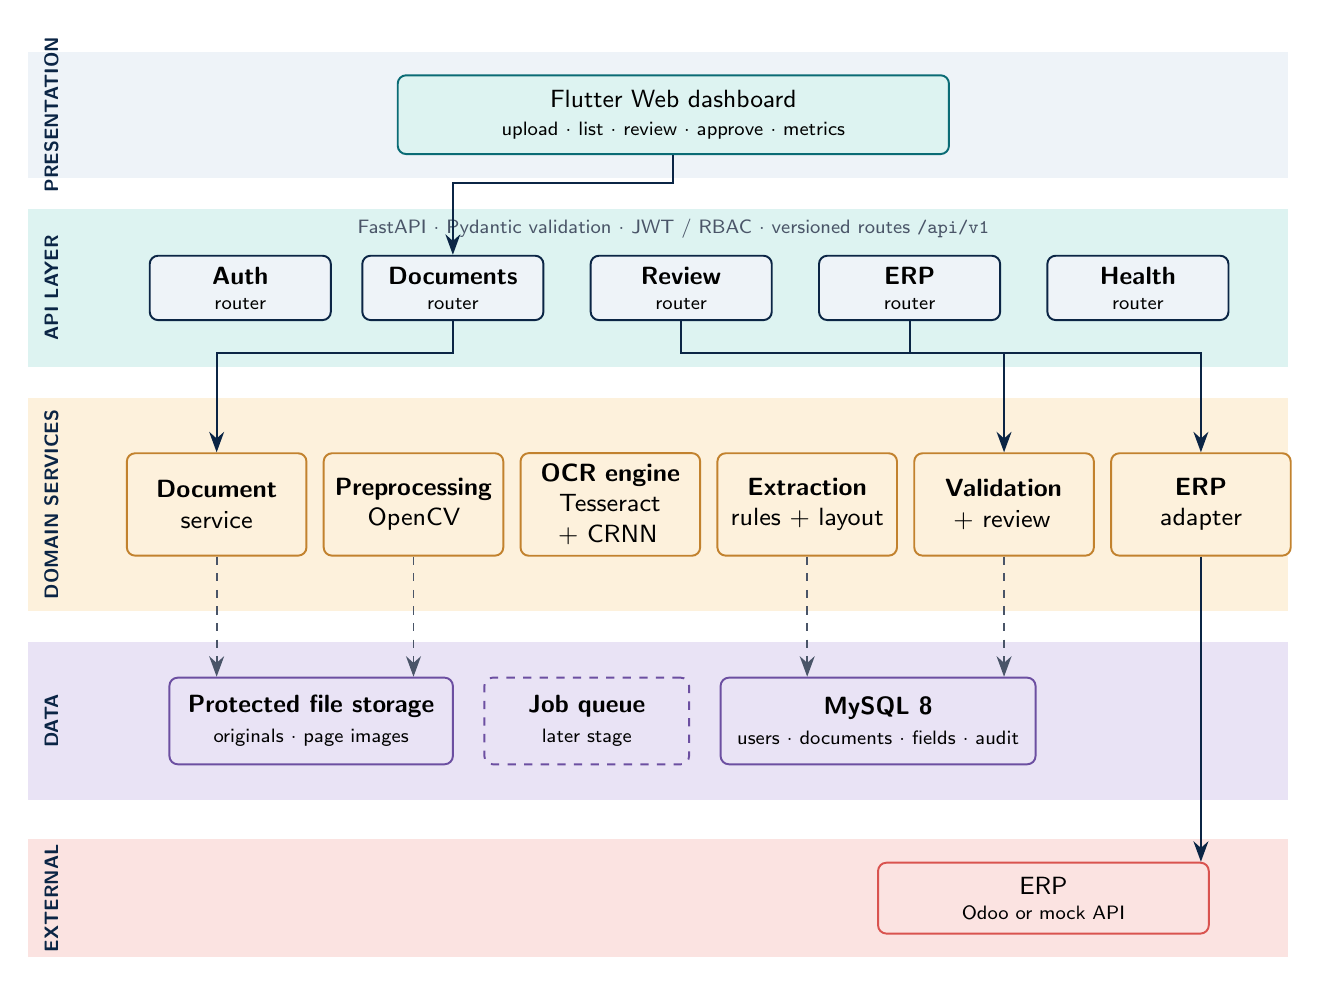
\begin{tikzpicture}[x=1cm,y=1cm]
% layer bands
\fill[mist]  (0,8.5) rectangle (16,10.1);
\fill[mint]  (0,6.1) rectangle (16,8.1);
\fill[sand]  (0,3.0) rectangle (16,5.7);
\fill[lilac] (0,0.6) rectangle (16,2.6);
\fill[blush] (0,-1.4) rectangle (16,0.1);
\node[rotate=90,font=\sffamily\scriptsize\bfseries,text=navy] at (0.3,9.3) {PRESENTATION};
\node[rotate=90,font=\sffamily\scriptsize\bfseries,text=navy] at (0.3,7.1) {API LAYER};
\node[rotate=90,font=\sffamily\scriptsize\bfseries,text=navy] at (0.3,4.35) {DOMAIN SERVICES};
\node[rotate=90,font=\sffamily\scriptsize\bfseries,text=navy] at (0.3,1.6) {DATA};
\node[rotate=90,font=\sffamily\scriptsize\bfseries,text=navy] at (0.3,-0.65) {EXTERNAL};
% presentation
\node[boxT,minimum width=7cm,minimum height=1cm] (ui) at (8.2,9.3) {Flutter Web dashboard\\[-1pt]\scriptsize upload $\cdot$ list $\cdot$ review $\cdot$ approve $\cdot$ metrics};
% api
\foreach \x/\t in {2.3/Auth,5.0/Documents,7.9/Review,10.8/ERP,13.7/Health}{
  \node[box,minimum width=2.3cm] (r\t) at (\x+0.4,7.1) {\textbf{\t}\\[-2pt]\scriptsize router};}
\node[font=\sffamily\scriptsize,text=slate] at (8.2,7.85) {FastAPI $\cdot$ Pydantic validation $\cdot$ JWT / RBAC $\cdot$ versioned routes \texttt{/api/v1}};
% domain
\foreach \x/\t/\s in {2.3/Document/service,4.95/Pre-/processing,7.6/OCR/engine,10.25/Extraction/rules,12.9/Validation/+ review,15.0/ERP/adapter}{}
\node[boxA,text width=2.0cm,minimum height=1.3cm] (sdoc) at (2.4,4.35)  {\textbf{Document}\\service};
\node[boxA,text width=2.0cm,minimum height=1.3cm] (spre) at (4.9,4.35)  {\textbf{Preprocessing}\\OpenCV};
\node[boxA,text width=2.0cm,minimum height=1.3cm] (socr) at (7.4,4.35)  {\textbf{OCR engine}\\Tesseract\\+ CRNN};
\node[boxA,text width=2.0cm,minimum height=1.3cm] (sext) at (9.9,4.35)  {\textbf{Extraction}\\rules + layout};
\node[boxA,text width=2.0cm,minimum height=1.3cm] (sval) at (12.4,4.35) {\textbf{Validation}\\+ review};
\node[boxA,text width=2.0cm,minimum height=1.3cm] (serp) at (14.9,4.35) {\textbf{ERP}\\adapter};
% data
\node[boxV,minimum width=3.6cm,minimum height=1.1cm] (fs) at (3.6,1.6) {\textbf{Protected file storage}\\\scriptsize originals $\cdot$ page images};
\node[boxV,minimum width=2.6cm,minimum height=1.1cm,dashed] (q) at (7.1,1.6) {\textbf{Job queue}\\\scriptsize later stage};
\node[boxV,minimum width=4.0cm,minimum height=1.1cm] (db) at (10.8,1.6) {\textbf{MySQL 8}\\\scriptsize users $\cdot$ documents $\cdot$ fields $\cdot$ audit};
% external
\node[boxC,minimum width=4.2cm,minimum height=0.9cm] (erp) at (12.9,-0.65) {ERP\\[-2pt]\scriptsize Odoo or mock API};
% arrows
\draw[arr] (ui.south) -- ++(0,-0.35) -| (rDocuments.north);
\draw[arr] (rDocuments.south) -- ++(0,-0.4) -| (sdoc.north);
\draw[arr] (rReview.south) -- ++(0,-0.4) -| (sval.north);
\draw[arr] (rERP.south) -- ++(0,-0.4) -| (serp.north);
\draw[arrd] (sdoc.south) -- (sdoc.south |- fs.north);
\draw[arrd] (spre.south) -- (spre.south |- fs.north);
\draw[arrd] (sext.south) -- (sext.south |- db.north);
\draw[arrd] (sval.south) -- (sval.south |- db.north);
\draw[arr]  (serp.south) -- (serp.south |- erp.north);
\end{tikzpicture}
}
\caption{Layered logical architecture. Solid arrows are requests; dashed arrows are data access. The job queue is introduced only in a later stage.}\label{fig:arch}
\end{figure}

\section{Logical Modules}
{\tblstart\small
\begin{longtable}{L{3.0cm}L{6.2cm}L{4.7cm}}
\hdrrow \hdr{Module} & \hdr{Responsibilities} & \hdr{Input $\rightarrow$ output}\\ \endhead
Flutter Web UI & Sign-in, upload, document list, review workspace, status dashboard. & User actions $\rightarrow$ API calls and views.\\
API layer & Request validation, routing, authentication, consistent errors, API versioning. & HTTP/JSON.\\
Authentication & User identity, roles, token lifecycle, account status. & Credentials $\rightarrow$ principal.\\
Document service & Upload validation, metadata, storage reference, job lifecycle. & File $\rightarrow$ document ID and state.\\
Preprocessing / OCR & PDF rendering, image enhancement, line segmentation, recognition. & Page $\rightarrow$ text, regions, confidence.\\
Extraction & Turn OCR output into typed invoice fields and keep source evidence. & Text + layout $\rightarrow$ candidate fields.\\
Validation / review & Business rules, confidence policy, corrections, approvals. & Candidates $\rightarrow$ approved record.\\
ERP adapter & Map approved records, authenticate, submit, reconcile status. & Record $\rightarrow$ ERP response.\\
MySQL & Users, metadata, fields, workflow states, attempts, audit records. & Transactional data.\\
Protected storage & Original uploads and derived page images outside the web root. & Files.\\
\hline
\end{longtable}}

\section{Why Start with a Modular Monolith?}
Microservices add network calls, inter-service authentication, distributed failure modes and deployment effort. For a student project the sound path is to build clearly separated modules inside one backend, test their interfaces, and extract services only where needed (typically the OCR worker first, because it is slow and resource-hungry). This keeps the service-oriented design while the first milestone stays achievable. Chapter~\ref{ch:deploy} shows the Docker Compose and Kubernetes stages.

\section{Repository Structure}
\begin{lstlisting}[language=bash]
intelligent-document-processing/
  backend/
    app/
      main.py
      api/              # routers (health, auth, documents, review, erp)
      core/             # settings, security, logging
      database/         # engine, sessions
      models/           # SQLAlchemy models
      schemas/          # Pydantic schemas
      services/         # documents, preprocessing, ocr, extraction,
                        # validation, integration
      workers/          # background jobs (later)
    alembic/            # migrations
    tests/
    Dockerfile  requirements.txt
  frontend/flutter_app/
  ml/                   # datasets (not committed), training, evaluation
  infrastructure/       # docker, compose, kubernetes
  docs/
  docker-compose.yml  .env.example  README.md
\end{lstlisting}

\chapter{UML Modelling}\label{ch:uml}
This chapter presents the system from several standard UML viewpoints. Each diagram answers a different question: who uses the system (use cases), what it stores (class and ER), how a document changes state, how work flows, and how components talk to each other (sequence).

\section{Use-Case Diagram}
\begin{figure}[H]\centering
\resizebox{\textwidth}{!}{\begin{tikzpicture}[x=1cm,y=1cm]
\draw[rounded corners=6pt,fill=mist,draw=navy,line width=0.8pt] (3.0,-0.4) rectangle (14.0,10.9);
\node[font=\sffamily\bfseries\small,text=navy] at (8.5,10.5) {\projname{} system};
\node[ucase,minimum width=4.4cm] (u1) at (6.6,9.3)  {Upload document};
\node[ucase,minimum width=4.4cm] (u2) at (6.6,8.0)  {Track status and search documents};
\node[ucase,minimum width=4.4cm] (u3) at (6.6,6.7)  {Review and correct fields};
\node[ucase,minimum width=4.4cm] (u4) at (6.6,5.4)  {Approve or reject record};
\node[ucase,minimum width=4.4cm] (u5) at (6.6,4.1)  {Submit approved record to ERP};
\node[ucase,minimum width=4.4cm] (u6) at (6.6,2.8)  {View audit trail and metrics};
\node[ucase,minimum width=4.4cm] (u7) at (6.6,1.5)  {Configure rules and thresholds};
\node[ucase,minimum width=4.4cm] (u8) at (6.6,0.2)  {Manage users and roles};
\node[ucase,minimum width=2.3cm,fill=sand,draw=amber!80!black] (v1) at (12.2,9.3) {Validate file};
\node[ucase,minimum width=2.3cm,fill=sand,draw=amber!80!black] (v2) at (12.2,4.1) {Validate ERP payload};
\draw[arrd] (u1) -- node[lbl,above]{\stereo{include}} (v1);
\draw[arrd] (u5) -- node[lbl,above]{\stereo{include}} (v2);
\actor{op}{1.2}{8.1}{Document\\operator}
\actor{rv}{1.2}{4.8}{Reviewer /\\accountant}
\actor{ad}{1.2}{1.0}{Administrator /\\supervisor}
\node[box,fill=blush,draw=coral,minimum width=1.9cm,minimum height=1.4cm,align=center] (erp) at (15.9,4.1) {\stereo{system}\\\textbf{ERP / Odoo}\\(or mock API)};
\foreach \a/\u in {op/u1,op/u2, rv/u2,rv/u3,rv/u4, ad/u6,ad/u7,ad/u8, rv/u6}{\draw[color=navy,line width=0.6pt] (\a) -- (\u);}
\draw[color=navy,line width=0.6pt] (erp.west) -- (14.0,4.1) -- (v2.east);
\end{tikzpicture}
}
\caption{Use cases and actors. Every use case requires the user to be signed in (FR-01). \stereo{include} marks behaviour that is always executed as part of another use case.}\label{fig:usecase}
\end{figure}

\subsection*{Use-case summary}
{\tblstart\small
\begin{longtable}{L{4.2cm}L{3.1cm}L{6.5cm}}
\hdrrow \hdr{Use case} & \hdr{Actor} & \hdr{Outcome}\\ \endhead
Upload document & Operator & A valid file is stored, a document ID is returned, a job is queued.\\
Track status and search & Operator, Reviewer & Current state and history of each permitted document.\\
Review and correct fields & Reviewer & Corrected values saved with reasons and audit events.\\
Approve or reject record & Reviewer & Record becomes APPROVED or REJECTED.\\
Submit approved record to ERP & ERP system & ERP reference stored; failures recorded and retryable.\\
View audit trail and metrics & Administrator, Reviewer & Traceable history and processing statistics.\\
Configure rules and thresholds & Administrator & Validation rules and review thresholds updated.\\
Manage users and roles & Administrator & Accounts created, deactivated, roles assigned.\\
\hline
\end{longtable}}

\section{Class Diagrams}
\subsection{Domain model}
\begin{figure}[H]\centering
\resizebox{\textwidth}{!}{\begin{tikzpicture}[x=1cm,y=1cm]
\node[uclass] (user) at (0,0) {\cname{User}\nodepart{two}
 +user\_id : UUID\\ +email : str\\ +password\_hash : str\\ +role : Role\\ +is\_active : bool
 \nodepart{three}+authenticate()\\ +has\_permission(p)};
\node[uclass] (run) at (5.8,0) {\cname{ProcessingRun}\nodepart{two}
 +run\_id : UUID\\ +model\_version : str\\ +preproc\_config : JSON\\ +started\_at, ended\_at\\ +error\_category : str
 \nodepart{three}+start()\\ +finish(status)};
\node[uclass] (fld) at (11.6,0) {\cname{ExtractedField}\nodepart{two}
 +field\_id : UUID\\ +name : str\\ +raw\_value, value : str\\ +confidence : float\\ +page, bbox : int[ ]\\ +validation : PASS|REVIEW|FAIL
 \nodepart{three}+correct(v, reason)};
\node[uclass] (doc) at (5.8,-5.0) {\cname{Document}\nodepart{two}
 +document\_id : UUID\\ +storage\_key : str\\ +sha256 : str\\ +mime\_type : str\\ +size\_bytes : int\\ +status : DocumentStatus\\ +created\_at : datetime
 \nodepart{three}+transition(to)\\ +is\_duplicate\_of(d)};
\node[uclass] (rev) at (0,-5.0) {\cname{Review}\nodepart{two}
 +review\_id : UUID\\ +decision : Decision\\ +notes : str\\ +decided\_at : datetime
 \nodepart{three}+approve()\\ +reject(reason)};
\node[uclass] (erp) at (11.6,-5.0) {\cname{ERPAttempt}\nodepart{two}
 +attempt\_id : UUID\\ +idempotency\_key : str\\ +destination : str\\ +status : str\\ +external\_ref : str\\ +error : str
 \nodepart{three}+submit(payload)\\ +retry()};
\node[uclass] (aud) at (5.8,-10.4) {\cname{AuditEvent}\nodepart{two}
 +event\_id : UUID\\ +actor\_id : UUID\\ +document\_id : UUID\\ +action : str\\ +before, after : JSON\\ +at : datetime
 \nodepart{three}+record(action, ctx)};
\node[uenum] (enum) at (11.6,-10.4) {\cname{\stereo{enum} DocumentStatus}\nodepart{two}
 UPLOADED, QUEUED,\\ PROCESSING, NEEDS\_REVIEW,\\ APPROVED, REJECTED,\\ ERP\_SENT, ERP\_FAILED, FAILED};
% relations
\draw[color=navy,line width=0.7pt] (user.south) -- node[lbl,pos=0.15,right]{1} node[lbl,pos=0.5,right]{reviews} node[lbl,pos=0.85,right]{0..*} (user.south |- rev.north);
\draw[color=navy,line width=0.7pt] (user.south east) -- node[lbl,pos=0.12,above right]{1} node[lbl,pos=0.5,sloped,above]{uploads} node[lbl,pos=0.88,above]{0..*} (doc.north west);
\draw[color=navy,line width=0.7pt] (doc.north) -- node[lbl,pos=0.1,left]{1} node[lbl,pos=0.5,left]{processed by} node[lbl,pos=0.9,left]{1..*} (run.south);
\draw[color=navy,line width=0.7pt,-{Diamond[open,length=3mm]}] (fld.west) -- node[lbl,pos=0.12,above]{0..*} node[lbl,pos=0.88,above]{1} (run.east);
\draw[color=navy,line width=0.7pt] (rev.east) -- node[lbl,pos=0.12,above]{0..*} node[lbl,pos=0.88,above]{1} (doc.west);
\draw[color=navy,line width=0.7pt] (doc.east) -- node[lbl,pos=0.12,above]{1} node[lbl,pos=0.88,above]{0..*} (erp.west);
\draw[color=navy,line width=0.7pt] (doc.south) -- node[lbl,pos=0.15,left]{1} node[lbl,pos=0.5,left]{logged in} node[lbl,pos=0.85,left]{0..*} (aud.north);
\draw[color=slate,dashed,line width=0.7pt,-{Stealth[open]}] (doc.south east) -- node[lbl,sloped,above]{uses} (enum.north west);
\end{tikzpicture}
}
\caption{Domain class diagram. A hollow diamond marks composition-like ownership (a processing run owns its extracted fields); plain lines are associations with multiplicities.}\label{fig:classdomain}
\end{figure}

\subsection{Service layer and extension points}
Two interfaces isolate the parts most likely to change. \texttt{OcrEngine} lets the pipeline use Tesseract (baseline) or the custom CRNN without modification, which is exactly what the comparison experiment needs. \texttt{ErpAdapter} keeps ERP-specific code (mock now, Odoo later) out of the document-processing logic (research question~5).
\begin{figure}[H]\centering
\resizebox{\textwidth}{!}{\begin{tikzpicture}[x=1cm,y=1cm]
\node[uclass2] (pipe) at (3.7,0) {\cname{ProcessingPipeline}\nodepart{two}
 +run(document\_id)\\ -preprocess(pages)\\ -recognize(image) : OcrResult\\ -extract(text) : Fields\\ -validate(fields) : Findings};
\node[uclass2] (integ) at (12.3,0) {\cname{IntegrationService}\nodepart{two}
 +submit(document\_id)\\ -build\_payload(record)\\ -idempotency\_key(record)\\ +retry(attempt\_id)};
\node[uiface] (ocr) at (3.7,-3.9) {\cname{\stereo{interface}\ OcrEngine}\nodepart{two}
 +recognize(image) : OcrResult\\ +name : str\\ +version : str};
\node[uiface] (erpa) at (12.3,-3.9) {\cname{\stereo{interface}\ ErpAdapter}\nodepart{two}
 +submit(payload) : ErpResult\\ +get\_status(ref) : Status};
\node[uclass2,text width=3.0cm] (tess) at (1.7,-7.4) {\cname{TesseractEngine}\nodepart{two}
 baseline OCR\\ (comparison)};
\node[uclass2,text width=3.0cm] (crnn) at (5.7,-7.4) {\cname{CrnnEngine}\nodepart{two}
 PyTorch CRNN + CTC\\ model\_version};
\node[uclass2,text width=3.0cm] (mock) at (10.5,-7.4) {\cname{MockErpAdapter}\nodepart{two}
 local test endpoint\\ simulates success/failure};
\node[uclass2,text width=3.0cm] (odoo) at (14.4,-7.4) {\cname{OdooAdapter}\nodepart{two}
 maps fields to Odoo\\ vendor bill (verified later)};
\draw[arrd] (pipe.south) -- node[lbl,right]{uses} (ocr.north);
\draw[arrd] (integ.south) -- node[lbl,right]{uses} (erpa.north);
\foreach \c/\i in {tess/ocr,crnn/ocr,mock/erpa,odoo/erpa}{
  \draw[color=slate,dashed,line width=0.7pt,-{Triangle[open,length=3.2mm,width=3mm]}] (\c.north) -- ++(0,0.6) -| (\i.south);}
\node[font=\sffamily\scriptsize,text=slate,text width=6.2cm,align=center] at (8.0,-9.4) {Dashed arrows with open heads show \emph{realization}: concrete engines and adapters implement the same interface, so either can be swapped without changing the pipeline.};
\end{tikzpicture}
}
\caption{Strategy pattern for OCR engines and ERP adapters.}\label{fig:classservices}
\end{figure}

\section{State Machine of a Document}
A document moves through explicit states. The implementation must reject invalid transitions (for example, an unreviewed document must never jump to \texttt{ERP\_SENT}).
\begin{figure}[H]\centering
\resizebox{0.95\textwidth}{!}{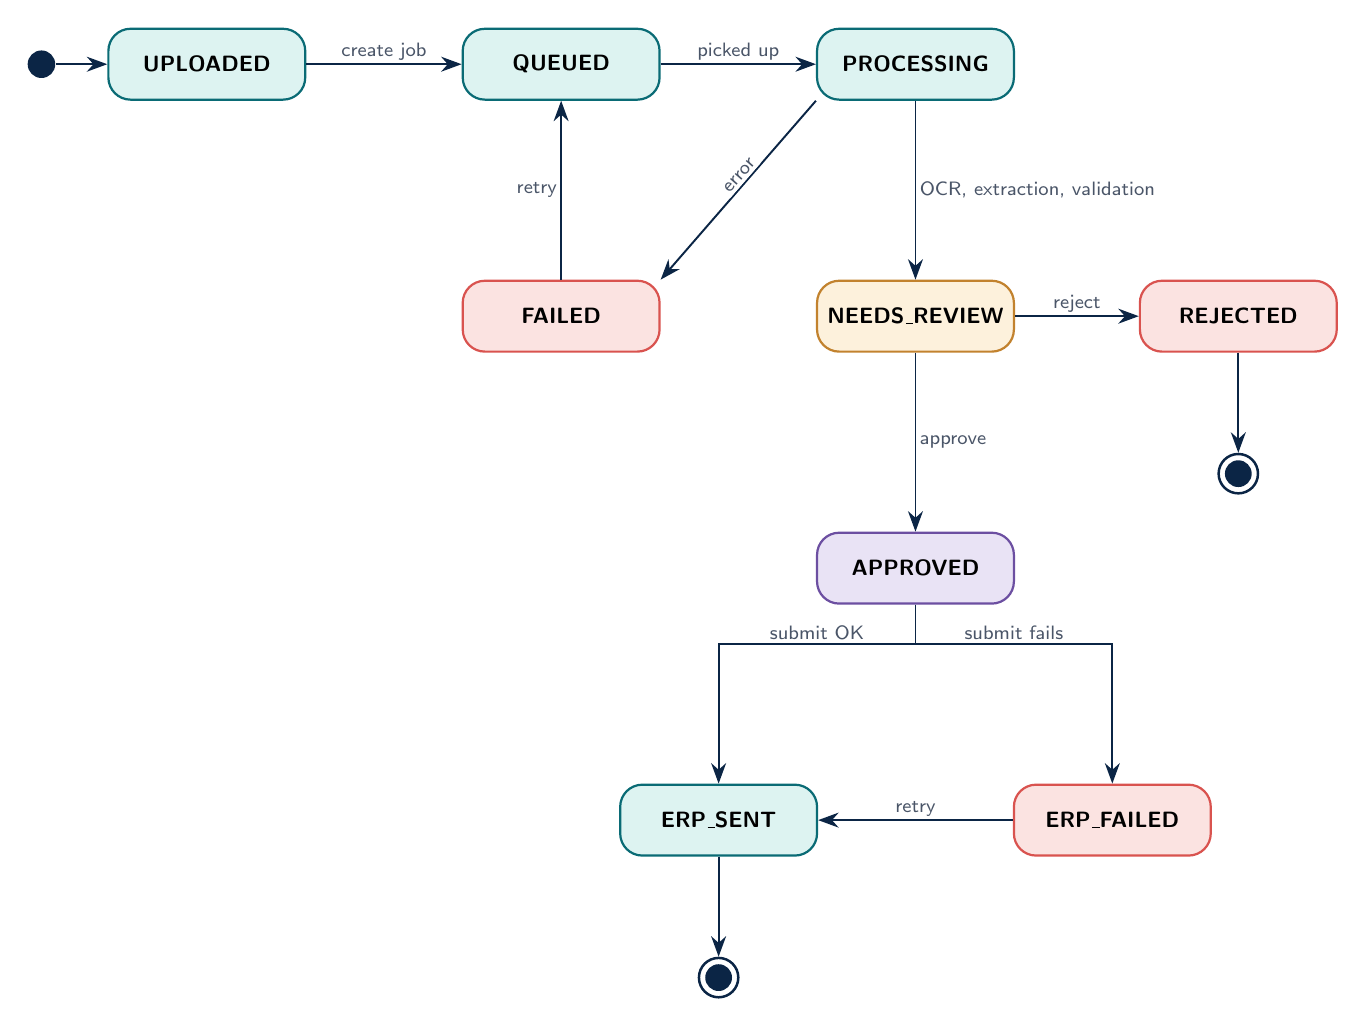
\begin{tikzpicture}[x=1cm,y=1cm]
\node[initial] (i) at (-0.6,0) {};
\node[state] (up) at (1.5,0) {UPLOADED};
\node[state] (qu) at (6.0,0) {QUEUED};
\node[state] (pr) at (10.5,0) {PROCESSING};
\node[stateC] (fa) at (6.0,-3.2) {FAILED};
\node[stateA] (nr) at (10.5,-3.2) {NEEDS\_REVIEW};
\node[stateC] (rj) at (14.6,-3.2) {REJECTED};
\node[stateV] (ap) at (10.5,-6.4) {APPROVED};
\node[state] (es) at (8.0,-9.6) {ERP\_SENT};
\node[stateC] (ef) at (13.0,-9.6) {ERP\_FAILED};
\node[final] (f) at (8.0,-11.6) {};
\node[final] (f2) at (14.6,-5.2) {};
\draw[arr] (i) -- (up);
\draw[arr] (up) -- node[lbl,above]{create job} (qu);
\draw[arr] (qu) -- node[lbl,above]{picked up} (pr);
\draw[arr] (pr) -- node[lbl,right]{OCR, extraction, validation} (nr);
\draw[arr] (pr.south west) -- node[lbl,above,sloped,pos=0.45]{error} (fa.north east);
\draw[arr] (fa) -- node[lbl,left]{retry} (qu);
\draw[arr] (nr) -- node[lbl,above]{reject} (rj);
\draw[arr] (rj) -- (f2);
\draw[arr] (nr) -- node[lbl,right]{approve} (ap);
\draw[arr] (ap.south) -- ++(0,-0.5) -| node[lbl,pos=0.25,above]{submit OK} (es.north);
\draw[arr] (ap.south) -- ++(0,-0.5) -| node[lbl,pos=0.25,above]{submit fails} (ef.north);
\draw[arr] (ef) -- node[lbl,above]{retry} (es);
\draw[arr] (es) -- (f);
\end{tikzpicture}
}
\caption{Document lifecycle. Initial state is the filled dot; double circles are final states.}\label{fig:state}
\end{figure}

{\tblstart\small
\begin{longtable}{L{3.4cm}L{3.4cm}L{7.0cm}}
\hdrrow \hdr{From} & \hdr{To} & \hdr{Trigger / guard}\\ \endhead
UPLOADED & QUEUED & Upload accepted and stored.\\
QUEUED & PROCESSING & Worker starts a processing run.\\
PROCESSING & NEEDS\_REVIEW & Extraction and validation complete (human approval is mandatory in the prototype).\\
PROCESSING & FAILED & Unrecoverable step error; error category stored.\\
FAILED & QUEUED & Manual or bounded automatic retry (FR-21).\\
NEEDS\_REVIEW & APPROVED / REJECTED & Authorised reviewer decision.\\
REJECTED & QUEUED & Reprocessing requested; creates a new run (FR-21).\\
APPROVED & ERP\_SENT / ERP\_FAILED & ERP response.\\
ERP\_FAILED & ERP\_SENT & Retry with the same idempotency key.\\
\hline
\end{longtable}}

\section{Activity Diagram}
\begin{figure}[H]\centering
\resizebox{!}{0.66\textheight}{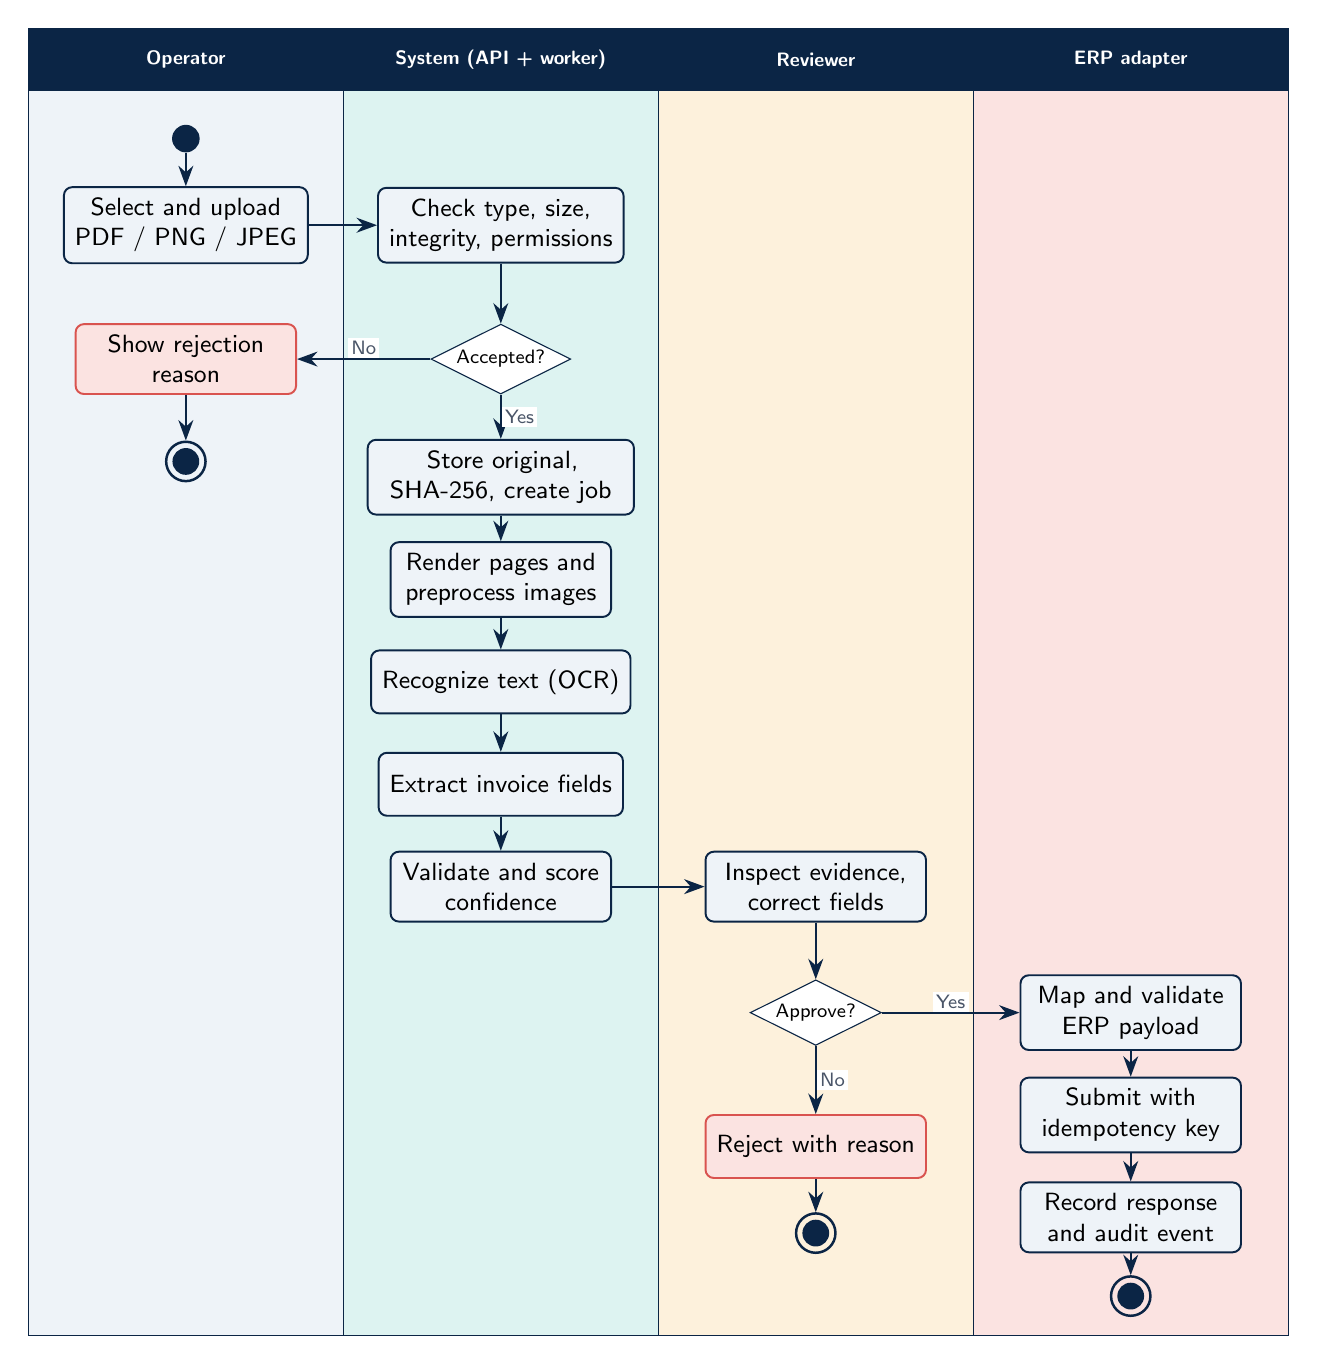
\begin{tikzpicture}[x=1cm,y=1cm]
% lanes
\foreach \x/\t/\c in {0/Operator/mist, 4/System (API + worker)/mint, 8/Reviewer/sand, 12/ERP adapter/blush}{
  \fill[\c] (\x,-16.4) rectangle (\x+4,0.2);
  \draw[navy,line width=0.5pt] (\x,-16.4) rectangle (\x+4,0.2);
  \fill[navy] (\x,-0.6) rectangle (\x+4,0.2);
  \node[text=white,font=\sffamily\bfseries\scriptsize] at (\x+2,-0.2) {\t};}
% nodes
\node[initial] (s) at (2,-1.2) {};
\node[box,minimum width=2.8cm] (a1) at (2,-2.3) {Select and upload\\ PDF / PNG / JPEG};
\node[box,minimum width=2.8cm] (a2) at (6,-2.3) {Check type, size,\\ integrity, permissions};
\node[diamond,aspect=2,draw=navy,fill=white,inner sep=1pt,font=\sffamily\scriptsize,align=center] (d1) at (6,-4.0) {Accepted?};
\node[box,minimum width=2.8cm,fill=blush,draw=coral] (a3) at (2,-4.0) {Show rejection\\ reason};
\node[final] (e1) at (2,-5.3) {};
\node[box,minimum width=2.8cm,text width=3.1cm] (a4) at (6,-5.5) {Store original, SHA-256, create job};
\node[box,minimum width=2.8cm] (a5) at (6,-6.8) {Render pages and\\ preprocess images};
\node[box,minimum width=2.8cm] (a6) at (6,-8.1) {Recognize text (OCR)};
\node[box,minimum width=2.8cm] (a7) at (6,-9.4) {Extract invoice fields};
\node[box,minimum width=2.8cm] (a8) at (6,-10.7) {Validate and score\\ confidence};
\node[box,minimum width=2.8cm] (b1) at (10,-10.7) {Inspect evidence,\\ correct fields};
\node[diamond,aspect=2,draw=navy,fill=white,inner sep=1pt,font=\sffamily\scriptsize,align=center] (d2) at (10,-12.3) {Approve?};
\node[box,minimum width=2.8cm,fill=blush,draw=coral] (b2) at (10,-14.0) {Reject with reason};
\node[final] (e2) at (10,-15.1) {};
\node[box,minimum width=2.8cm] (c1) at (14,-12.3) {Map and validate\\ ERP payload};
\node[box,minimum width=2.8cm] (c2) at (14,-13.6) {Submit with\\ idempotency key};
\node[box,minimum width=2.8cm] (c3) at (14,-14.9) {Record response\\ and audit event};
\node[final] (e3) at (14,-15.9) {};
% edges
\draw[arr] (s) -- (a1);
\draw[arr] (a1) -- (a2.west);
\draw[arr] (a2) -- (d1);
\draw[arr] (d1.west) -- node[lbl,above]{No} (a3.east);
\draw[arr] (a3) -- (e1);
\draw[arr] (d1) -- node[lbl,right]{Yes} (a4);
\foreach \a/\b in {a4/a5,a5/a6,a6/a7,a7/a8}{\draw[arr] (\a) -- (\b);}
\draw[arr] (a8) -- (b1);
\draw[arr] (b1) -- (d2);
\draw[arr] (d2) -- node[lbl,right]{No} (b2);
\draw[arr] (b2) -- (e2);
\draw[arr] (d2.east) -- node[lbl,above]{Yes} (c1.west);
\draw[arr] (c1) -- (c2);
\draw[arr] (c2) -- (c3);
\draw[arr] (c3) -- (e3);
\end{tikzpicture}
}
\caption{Swimlane activity diagram from upload to controlled ERP submission. Rejection ends the workflow without any ERP call.}\label{fig:activity}
\end{figure}

\section{Sequence Diagrams}
\begin{figure}[H]\centering
\resizebox{\textwidth}{!}{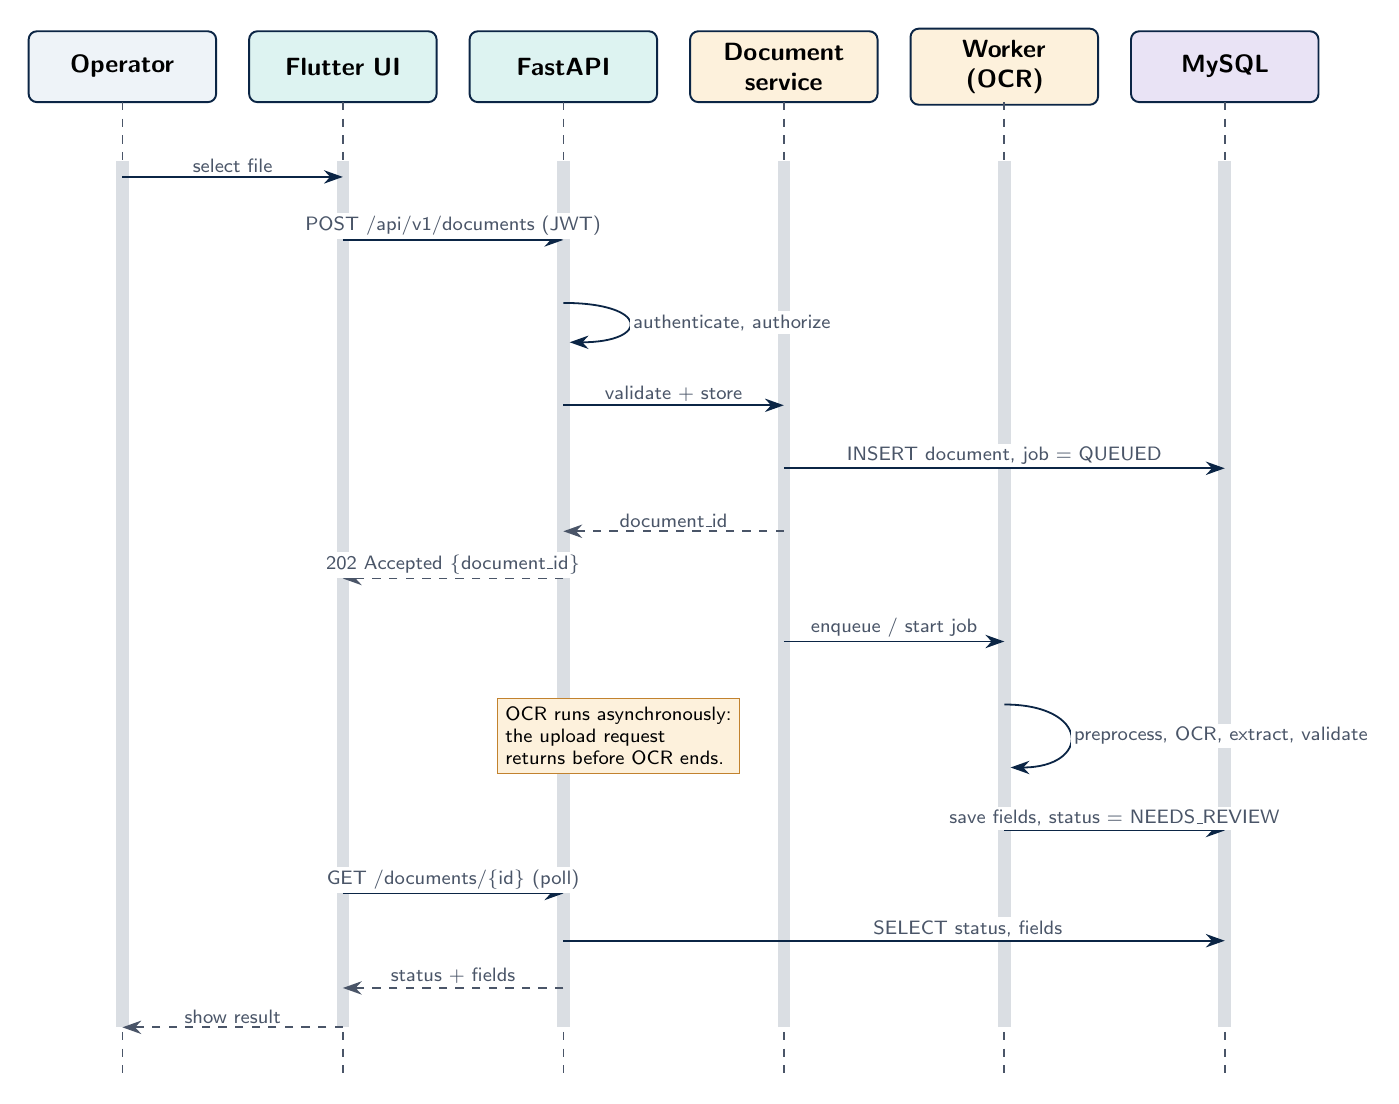
\begin{tikzpicture}[x=1cm,y=1cm]
\def\ys{-0.9}
\foreach \x/\n/\c in {0.9/Operator/mist, 3.7/Flutter UI/mint, 6.5/FastAPI/mint, 9.3/Document\\service/sand, 12.1/Worker\\(OCR)/sand, 14.9/MySQL/lilac}{
  \node[box,fill=\c,minimum width=2.3cm,text width=2.1cm,minimum height=0.9cm] (p\x) at (\x,0) {\textbf{\n}};
  \draw[lifeline] (\x,-0.45) -- (\x,-12.8);
  \fill[navy!15] (\x-0.08,-1.2) rectangle (\x+0.08,-12.2);}
% messages (y descending)
\draw[msg] (0.9,-1.4) -- node[lbl,above]{select file} (3.7,-1.4);
\draw[msg] (3.7,-2.2) -- node[lbl,above]{POST /api/v1/documents (JWT)} (6.5,-2.2);
\draw[msg] (6.5,-3.0) .. controls (7.6,-3.0) and (7.6,-3.5) .. node[lbl,right,pos=0.5]{authenticate, authorize} (6.58,-3.5);
\draw[msg] (6.5,-4.3) -- node[lbl,above]{validate + store} (9.3,-4.3);
\draw[msg] (9.3,-5.1) -- node[lbl,above]{INSERT document, job = QUEUED} (14.9,-5.1);
\draw[ret] (9.3,-5.9) -- node[lbl,above]{document\_id} (6.5,-5.9);
\draw[ret] (6.5,-6.5) -- node[lbl,above]{202 Accepted \{document\_id\}} (3.7,-6.5);
\draw[msg] (9.3,-7.3) -- node[lbl,above]{enqueue / start job} (12.1,-7.3);
\draw[msg] (12.1,-8.1) .. controls (13.2,-8.1) and (13.2,-8.9) .. node[lbl,right,pos=0.5]{preprocess, OCR, extract, validate} (12.18,-8.9);
\draw[msg] (12.1,-9.7) -- node[lbl,above]{save fields, status = NEEDS\_REVIEW} (14.9,-9.7);
\draw[msg] (3.7,-10.5) -- node[lbl,above]{GET /documents/\{id\} (poll)} (6.5,-10.5);
\draw[msg] (6.5,-11.1) .. controls (10.7,-11.1) and (13.2,-11.1) .. node[lbl,above,pos=0.5]{SELECT status, fields} (14.9,-11.1);
\draw[ret] (6.5,-11.7) -- node[lbl,above]{status + fields} (3.7,-11.7);
\draw[ret] (3.7,-12.2) -- node[lbl,above]{show result} (0.9,-12.2);
% async note
\node[draw=amber!80!black,fill=sand,font=\sffamily\scriptsize,align=left,inner sep=3pt] at (7.2,-8.5) {OCR runs asynchronously:\\ the upload request\\ returns before OCR ends.};
\end{tikzpicture}
}
\caption{Upload to OCR result. The upload request returns before OCR finishes; the UI polls the status endpoint.}\label{fig:sequpload}
\end{figure}

\begin{figure}[H]\centering
\resizebox{\textwidth}{!}{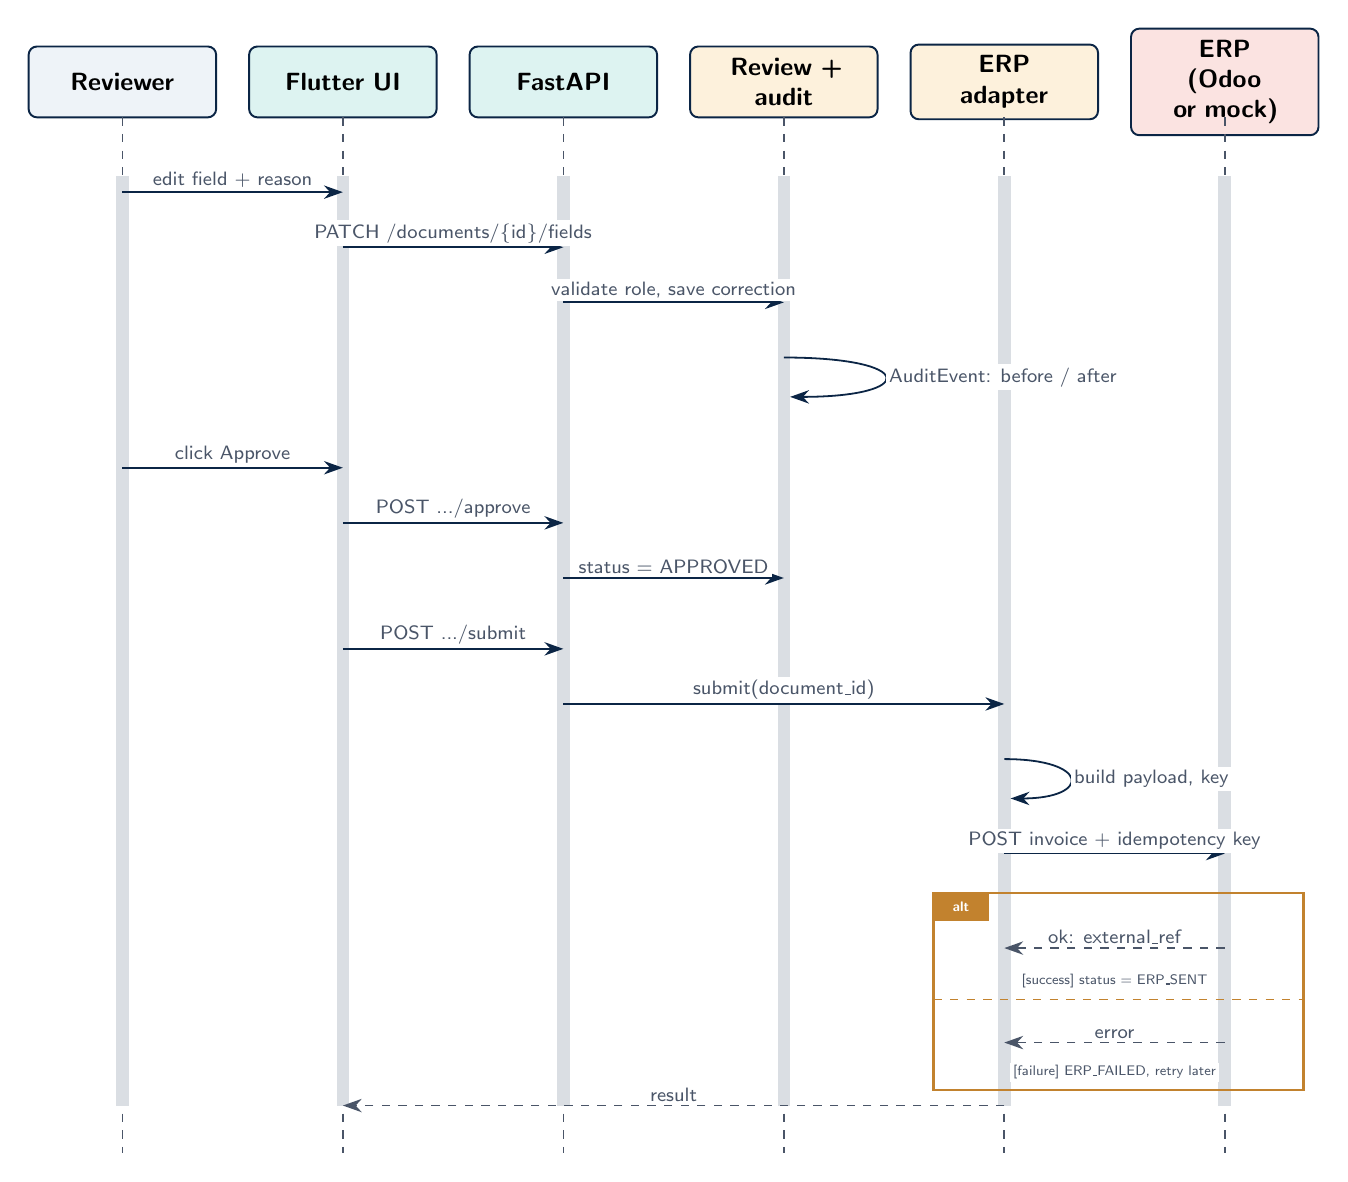
\begin{tikzpicture}[x=1cm,y=1cm]
\foreach \x/\n/\c in {0.9/Reviewer/mist, 3.7/Flutter UI/mint, 6.5/FastAPI/mint, 9.3/Review +\\audit/sand, 12.1/ERP\\adapter/sand, 14.9/ERP\\(Odoo or mock)/blush}{
  \node[box,fill=\c,minimum width=2.3cm,text width=2.1cm,minimum height=0.9cm] at (\x,0) {\textbf{\n}};
  \draw[lifeline] (\x,-0.45) -- (\x,-13.6);
  \fill[navy!15] (\x-0.08,-1.2) rectangle (\x+0.08,-13.0);}
\draw[msg] (0.9,-1.4) -- node[lbl,above]{edit field + reason} (3.7,-1.4);
\draw[msg] (3.7,-2.1) -- node[lbl,above]{PATCH /documents/\{id\}/fields} (6.5,-2.1);
\draw[msg] (6.5,-2.8) -- node[lbl,above]{validate role, save correction} (9.3,-2.8);
\draw[msg] (9.3,-3.5) .. controls (11,-3.5) and (11,-4.0) .. node[lbl,right,pos=0.5]{AuditEvent: before / after} (9.38,-4.0);
\draw[msg] (0.9,-4.9) -- node[lbl,above]{click Approve} (3.7,-4.9);
\draw[msg] (3.7,-5.6) -- node[lbl,above]{POST .../approve} (6.5,-5.6);
\draw[msg] (6.5,-6.3) -- node[lbl,above]{status = APPROVED} (9.3,-6.3);
\draw[msg] (3.7,-7.2) -- node[lbl,above]{POST .../submit} (6.5,-7.2);
\draw[msg] (6.5,-7.9) -- node[lbl,above]{submit(document\_id)} (12.1,-7.9);
\draw[msg] (12.1,-8.6) .. controls (13.2,-8.6) and (13.2,-9.1) .. node[lbl,right,pos=0.5]{build payload, key} (12.18,-9.1);
\draw[msg] (12.1,-9.8) -- node[lbl,above]{POST invoice + idempotency key} (14.9,-9.8);
% alt frame
\draw[amber!80!black,line width=0.8pt] (11.2,-10.3) rectangle (15.9,-12.8);
\fill[amber!80!black] (11.2,-10.3) rectangle (11.9,-10.65);
\node[text=white,font=\sffamily\bfseries\tiny] at (11.55,-10.47) {alt};
\draw[ret] (14.9,-11.0) -- node[lbl,above]{ok: external\_ref} (12.1,-11.0);
\node[font=\sffamily\tiny,text=slate,fill=white,inner sep=1pt] at (13.5,-11.42) {[success] status = ERP\_SENT};
\draw[dashed,amber!80!black] (11.2,-11.65) -- (15.9,-11.65);
\draw[ret] (14.9,-12.2) -- node[lbl,above]{error} (12.1,-12.2);
\node[font=\sffamily\tiny,text=slate,fill=white,inner sep=1pt] at (13.5,-12.58) {[failure] ERP\_FAILED, retry later};
\draw[ret] (12.1,-13.0) -- node[lbl,above]{result} (3.7,-13.0);
\end{tikzpicture}
}
\caption{Review, approval and ERP submission, including the success and failure branches of the integration call.}\label{fig:seqreview}
\end{figure}

\chapter{OCR, Extraction and Validation Design}
\section{OCR versus Document Understanding}
OCR identifies characters or words in an image. Extraction decides which recognised values correspond to business fields. Validation checks whether those values are plausible and consistent. Keeping these three stages separate lets each be tested independently.

\section{Processing Pipeline}
\begin{figure}[H]\centering
\resizebox{\textwidth}{!}{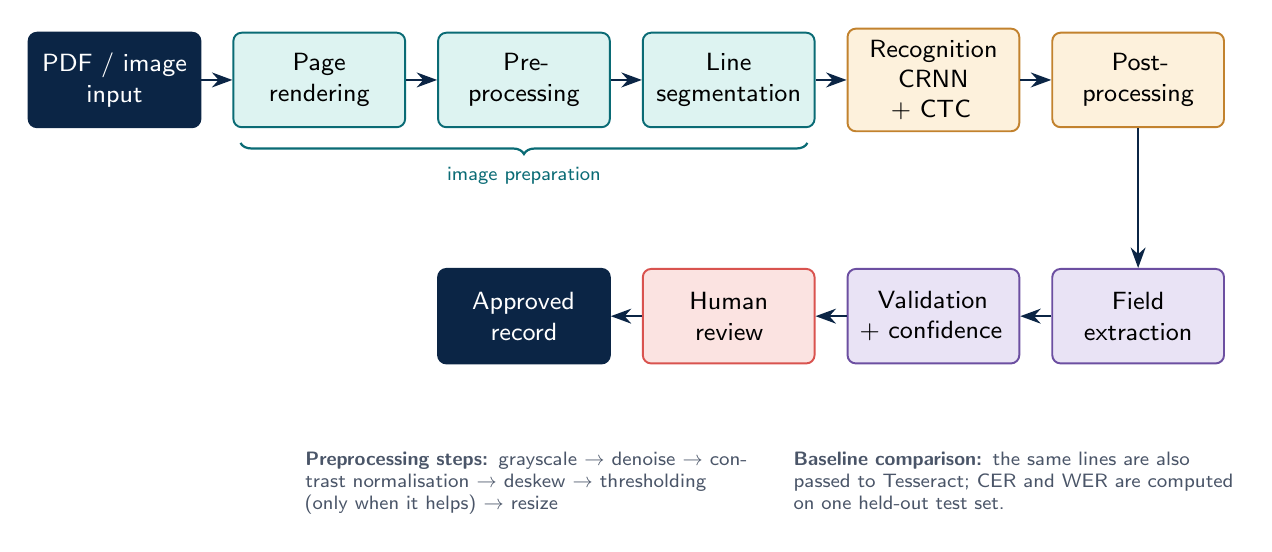
\begin{tikzpicture}[x=1cm,y=1cm,node distance=0.55cm]
\node[boxN,text width=1.9cm,minimum height=1.2cm] (n1) at (1.1,0) {PDF / image\\ input};
\node[boxT,text width=1.9cm,minimum height=1.2cm] (n2) at (3.7,0) {Page\\ rendering};
\node[boxT,text width=1.9cm,minimum height=1.2cm] (n3) at (6.3,0) {Pre-\\processing};
\node[boxT,text width=1.9cm,minimum height=1.2cm] (n4) at (8.9,0) {Line\\ segmentation};
\node[boxA,text width=1.9cm,minimum height=1.2cm] (n5) at (11.5,0) {Recognition\\ CRNN + CTC};
\node[boxA,text width=1.9cm,minimum height=1.2cm] (n6) at (14.1,0) {Post-\\processing};
\node[boxV,text width=1.9cm,minimum height=1.2cm] (n7) at (14.1,-3.0) {Field\\ extraction};
\node[boxV,text width=1.9cm,minimum height=1.2cm] (n8) at (11.5,-3.0) {Validation\\ + confidence};
\node[boxC,text width=1.9cm,minimum height=1.2cm] (n9) at (8.9,-3.0) {Human\\ review};
\node[boxN,text width=1.9cm,minimum height=1.2cm] (n10) at (6.3,-3.0) {Approved\\ record};
\foreach \a/\b in {n1/n2,n2/n3,n3/n4,n4/n5,n5/n6,n6/n7,n7/n8,n8/n9,n9/n10}{\draw[arr] (\a) -- (\b);}
\node[font=\sffamily\scriptsize,text=slate,text width=5.6cm,align=left,anchor=north west] at (3.4,-4.6) {\textbf{Preprocessing steps:} grayscale $\rightarrow$ denoise $\rightarrow$ contrast normalisation $\rightarrow$ deskew $\rightarrow$ thresholding (only when it helps) $\rightarrow$ resize};
\node[font=\sffamily\scriptsize,text=slate,text width=5.6cm,align=left,anchor=north west] at (9.6,-4.6) {\textbf{Baseline comparison:} the same lines are also passed to Tesseract; CER and WER are computed on one held-out test set.};
\draw[decorate,decoration={brace,amplitude=4pt,mirror},color=tealdark,line width=0.8pt] (2.7,-0.8) -- (9.9,-0.8) node[midway,below=5pt,font=\sffamily\scriptsize,text=tealdark] {image preparation};
\end{tikzpicture}
}
\caption{End-to-end processing pipeline. The same segmented lines feed both the custom recogniser and the baseline engine.}\label{fig:pipeline}
\end{figure}
\begin{enumerate}
\item \textbf{Input inspection:} file type, page count, dimensions, rotation, basic quality.
\item \textbf{PDF rendering:} render each page at a suitable resolution while keeping the original file.
\item \textbf{Preprocessing:} grayscale, denoising, contrast normalisation, skew correction, thresholding when helpful, resizing.
\item \textbf{Text segmentation:} the first prototype uses a constrained line-based approach; complex layouts need more robust detection.
\item \textbf{Recognition:} a CRNN with CTC loss, or a justified alternative after experiments.
\item \textbf{Post-processing:} normalise whitespace and common confusions without silently altering source evidence.
\item \textbf{Field extraction:} labels, layout positions, patterns and rules propose invoice fields.
\item \textbf{Confidence and review:} combine confidence with validation outcomes and route uncertain cases to a reviewer.
\end{enumerate}

\section{Custom Recognition Model}
\begin{figure}[H]\centering
\resizebox{\textwidth}{!}{\begin{tikzpicture}[x=1cm,y=1cm]
\node[boxN,text width=2.2cm,minimum height=2.0cm] (in) at (1.3,0) {Text-line image\\[2pt]\scriptsize $1\times H\times W$\\ $H=32$ (fixed)};
\node[boxT,text width=2.6cm,minimum height=2.0cm] (cnn) at (4.7,0) {Convolutional\\ feature extractor\\[2pt]\scriptsize conv + BN + ReLU\\ + max-pool blocks};
\node[boxA,text width=2.4cm,minimum height=2.0cm] (seq) at (8.2,0) {Feature sequence\\[2pt]\scriptsize $T\times C$\\ (one vector per\\ horizontal step)};
\node[boxV,text width=2.4cm,minimum height=2.0cm] (rnn) at (11.5,0) {Bidirectional\\ LSTM $\times 2$\\[2pt]\scriptsize context in both\\ directions};
\node[boxC,text width=2.3cm,minimum height=2.0cm] (out) at (14.7,0) {Linear + softmax\\[2pt]\scriptsize $T\times(|\mathcal{A}|+1)$\\ incl. CTC blank};
\foreach \a/\b in {in/cnn,cnn/seq,seq/rnn,rnn/out}{\draw[arr] (\a) -- (\b);}
\node[boxN,text width=6.6cm,minimum height=1.0cm] (ctc) at (11.0,-3.0) {CTC training loss $\mathcal{L}=-\log P(y\mid x)$ \ $\vert$ \ greedy / beam decoding at inference};
\draw[arr] (out.south) -- ++(0,-0.4) -| (ctc.north);
\node[boxA,text width=4.4cm,minimum height=1.0cm] (txt) at (3.2,-3.0) {Recognised text: \emph{``Facture N\textdegree{} 2026-017''}};
\draw[arr] (ctc.west) -- (txt.east);
\node[font=\sffamily\scriptsize,text=slate,text width=15cm,align=left,anchor=north west] at (0.2,-4.2) {$\mathcal{A}$: alphabet of French and English letters (including accented letters), digits, punctuation and business symbols. Image height and layer sizes are design choices to be tuned experimentally.};
\end{tikzpicture}
}
\caption{CRNN recogniser with CTC loss. Dimensions are indicative and will be tuned experimentally.}\label{fig:crnn}
\end{figure}
A CRNN combines a convolutional feature extractor, a bidirectional recurrent layer for sequence context and a character classifier. CTC loss allows training without character-level alignment:
\[
\mathcal{L}_{\text{CTC}} = -\log P(y\mid x),
\]
where $x$ is the input line image and $y$ the target text. The alphabet must cover French and English letters (including accents), digits, punctuation and business symbols.

\subsection{Dataset requirements}
\begin{itemize}
\item Representative invoice images with verified transcriptions.
\item Training, validation and test sets separated \emph{by document or source}, not by random crops of the same page.
\item Clean and degraded examples: low contrast, skew, noise, different fonts, stamps and scan artefacts.
\item Metadata: language, document type, image size and preprocessing settings.
\item Personal or confidential content removed or protected; dataset, label and model versions tracked.
\end{itemize}

\subsection{Evaluation metrics}
Character error rate and word error rate are
\[
\mathrm{CER}=\frac{S+D+I}{N},\qquad \mathrm{WER}=\frac{S_w+D_w+I_w}{N_w},
\]
with substitutions $S$, deletions $D$, insertions $I$ and reference length $N$ (characters or words). Both models are evaluated on the same held-out set. A lower value is better, and no number is written into the final report before the experiment has been run.

\section{Field Extraction Strategy}
For invoices the candidate fields are supplier name and tax identifier, invoice number, invoice and due dates, currency, subtotal, tax, total and purchase-order reference (Phase~1 specification, Table of invoice fields). Regular expressions handle constrained patterns; keyword anchors (``Invoice No.'', ``Facture N\textdegree'') and page coordinates locate values; arithmetic rules cross-check amounts. Each field keeps the text span or coordinates that support it, which is what the review screen highlights (FR-22).

\section{Validation Rules}
{\tblstart\small
\begin{longtable}{L{3.0cm}L{6.3cm}L{4.5cm}}
\hdrrow \hdr{Rule} & \hdr{Example check} & \hdr{Outcome}\\ \endhead
Required fields & Invoice number, supplier, date and total are present. & Missing field becomes a review finding.\\
Date parsing & Date parses under configured formats and a plausible range. & Invalid or ambiguous date flagged.\\
Numeric parsing & Amounts normalised using locale conventions (space or dot thousands). & Unparseable amount flagged.\\
Arithmetic & Subtotal + tax $\approx$ total within a configured tolerance. & Mismatch flagged, never auto-corrected.\\
Currency & Symbols and codes agree across fields. & Inconsistency flagged.\\
Duplicate indicator & Supplier, invoice number, date, amount, optional file hash. & Likely duplicate flagged.\\
ERP schema & Approved values satisfy the ERP payload schema. & Invalid payload blocked before sending.\\
\hline
\end{longtable}}

\section{Confidence Policy}
Confidence is a decision signal, not a guarantee. Thresholds are set empirically on validation data, never on the test set. A possible policy: high-confidence fields without rule violations are shown as accepted; medium-confidence fields are highlighted; low-confidence fields and critical validation failures require human review. In the prototype, human approval before ERP submission is mandatory.

\chapter{Data Design}
\section{Principles}
MySQL stores structured application data, not public copies of uploaded files. Originals live in protected storage (a private directory in development, private object storage in deployment). The database keeps the storage key, checksum, file metadata, status, extracted fields and audit data. File contents are never placed in a public web directory and internal paths are never exposed by the API.

\section{Entity-Relationship Diagram}
\begin{figure}[H]\centering
\resizebox{\textwidth}{!}{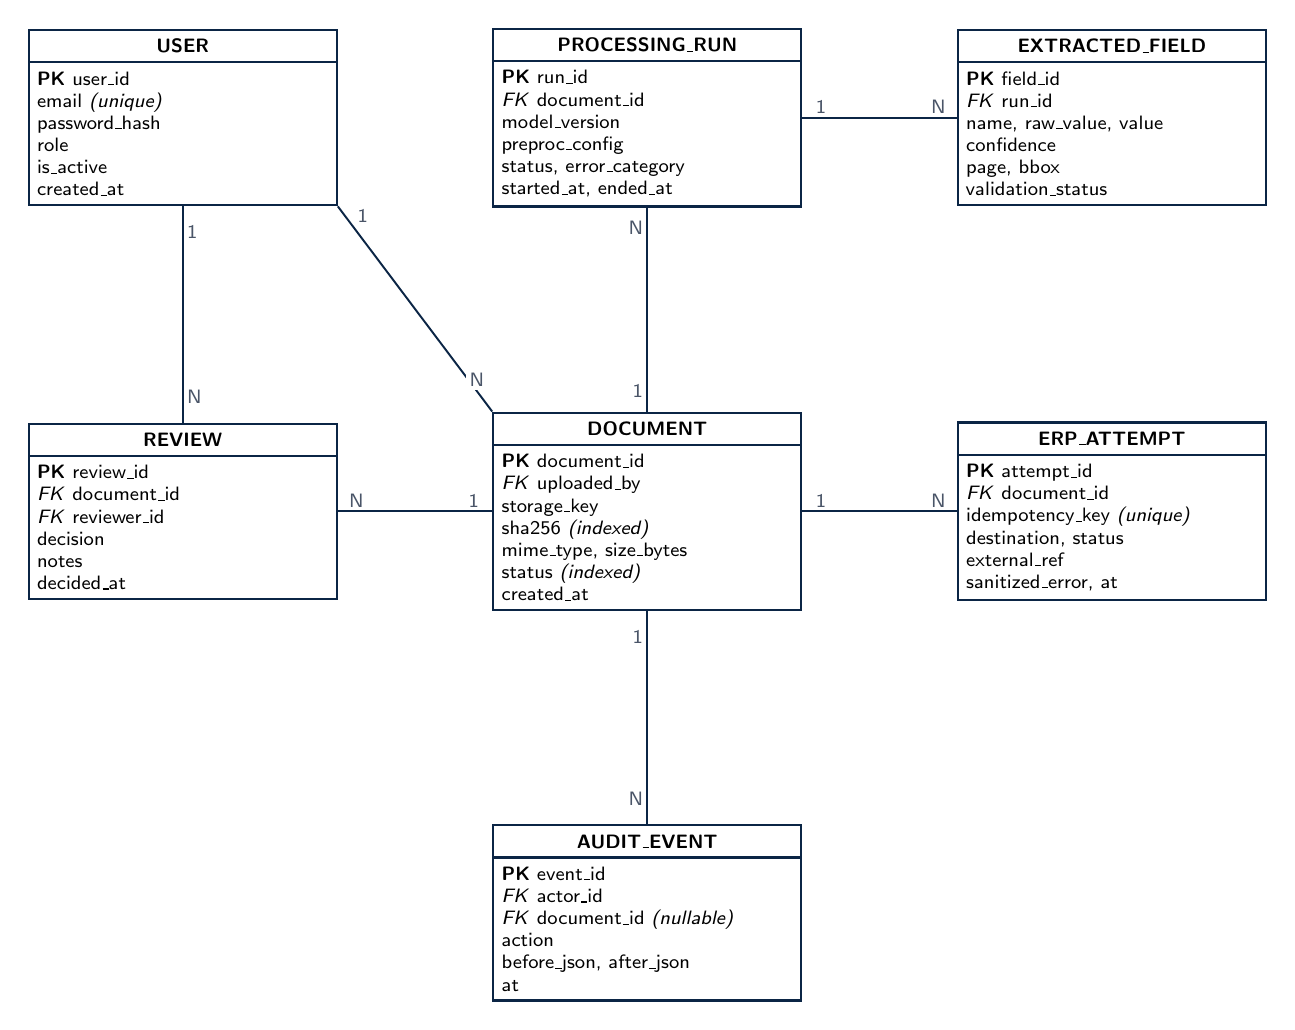
\begin{tikzpicture}[x=1cm,y=1cm,
  ent/.style={uclass2,text width=3.7cm},
  pk/.style={font=\bfseries},]
\node[ent] (user) at (0,0) {\centerline{{\bfseries USER}}\nodepart{two}
 \textbf{PK} user\_id\\ email \textit{(unique)}\\ password\_hash\\ role\\ is\_active\\ created\_at};
\node[ent] (run) at (5.9,0) {\centerline{{\bfseries PROCESSING\_RUN}}\nodepart{two}
 \textbf{PK} run\_id\\ \textit{FK} document\_id\\ model\_version\\ preproc\_config\\ status, error\_category\\ started\_at, ended\_at};
\node[ent] (fld) at (11.8,0) {\centerline{{\bfseries EXTRACTED\_FIELD}}\nodepart{two}
 \textbf{PK} field\_id\\ \textit{FK} run\_id\\ name, raw\_value, value\\ confidence\\ page, bbox\\ validation\_status};
\node[ent] (doc) at (5.9,-5.0) {\centerline{{\bfseries DOCUMENT}}\nodepart{two}
 \textbf{PK} document\_id\\ \textit{FK} uploaded\_by\\ storage\_key\\ sha256 \textit{(indexed)}\\ mime\_type, size\_bytes\\ status \textit{(indexed)}\\ created\_at};
\node[ent] (rev) at (0,-5.0) {\centerline{{\bfseries REVIEW}}\nodepart{two}
 \textbf{PK} review\_id\\ \textit{FK} document\_id\\ \textit{FK} reviewer\_id\\ decision\\ notes\\ decided\_at};
\node[ent] (erp) at (11.8,-5.0) {\centerline{{\bfseries ERP\_ATTEMPT}}\nodepart{two}
 \textbf{PK} attempt\_id\\ \textit{FK} document\_id\\ idempotency\_key \textit{(unique)}\\ destination, status\\ external\_ref\\ sanitized\_error, at};
\node[ent] (aud) at (5.9,-10.1) {\centerline{{\bfseries AUDIT\_EVENT}}\nodepart{two}
 \textbf{PK} event\_id\\ \textit{FK} actor\_id\\ \textit{FK} document\_id \textit{(nullable)}\\ action\\ before\_json, after\_json\\ at};
\tikzset{er/.style={color=navy,line width=0.7pt}}
\draw[er] (user.south) -- node[lbl,pos=0.12,right]{1} node[lbl,pos=0.88,right]{N} (user.south |- rev.north);
\draw[er] (user.south east) -- node[lbl,pos=0.1,above right]{1} node[lbl,pos=0.9,above]{N} (doc.north west);
\draw[er] (doc.north) -- node[lbl,pos=0.1,left]{1} node[lbl,pos=0.9,left]{N} (run.south);
\draw[er] (run.east) -- node[lbl,pos=0.12,above]{1} node[lbl,pos=0.88,above]{N} (fld.west);
\draw[er] (doc.west) -- node[lbl,pos=0.12,above]{1} node[lbl,pos=0.88,above]{N} (rev.east);
\draw[er] (doc.east) -- node[lbl,pos=0.12,above]{1} node[lbl,pos=0.88,above]{N} (erp.west);
\draw[er] (doc.south) -- node[lbl,pos=0.12,left]{1} node[lbl,pos=0.88,left]{N} (aud.north);
\end{tikzpicture}
}
\caption{Logical ER diagram (PK = primary key, FK = foreign key). Final constraints and indexes are fixed when the schema is implemented.}\label{fig:er}
\end{figure}

\section{Entity Descriptions}
{\tblstart\small
\begin{longtable}{L{3.0cm}L{10.8cm}}
\hdrrow \hdr{Entity} & \hdr{Purpose and key fields}\\ \endhead
User & Identity and role. A password hash is stored only if local passwords are used; never plaintext.\\
Document & One uploaded source document: storage key, SHA-256, MIME type, size, uploader, timestamps and current workflow status.\\
ProcessingRun & One attempt to process a document: preprocessing configuration, OCR model version, start/end time, status and error category.\\
ExtractedField & A candidate field of a run: name, raw and normalised value, confidence, page/region evidence and validation status.\\
Review & Human decision with reviewer, notes, timestamp and references to before/after values.\\
ERPAttempt & Each outbound attempt: idempotency key, destination, sanitised request/response metadata, external reference, status.\\
AuditEvent & Append-only record of upload, correction, approval, rejection, configuration changes and ERP submission.\\
\hline
\end{longtable}}

\section{Schema Excerpt}
The following MySQL excerpt illustrates intended constraints. It is a design sketch to be implemented with Alembic migrations, not a deployed schema.
\begin{lstlisting}[language=SQL]
CREATE TABLE documents (
  document_id  CHAR(36)     PRIMARY KEY,
  uploaded_by  CHAR(36)     NOT NULL,
  storage_key  VARCHAR(255) NOT NULL,
  sha256       CHAR(64)     NOT NULL,
  mime_type    VARCHAR(100) NOT NULL,
  size_bytes   BIGINT       NOT NULL,
  status       VARCHAR(20)  NOT NULL,
  created_at   TIMESTAMP    NOT NULL DEFAULT CURRENT_TIMESTAMP,
  FOREIGN KEY (uploaded_by) REFERENCES users(user_id),
  INDEX idx_documents_status (status),
  INDEX idx_documents_sha256 (sha256)
);
CREATE TABLE erp_attempts (
  attempt_id       CHAR(36)    PRIMARY KEY,
  document_id      CHAR(36)    NOT NULL,
  idempotency_key  VARCHAR(80) NOT NULL UNIQUE,
  status           VARCHAR(20) NOT NULL,
  external_ref     VARCHAR(100),
  FOREIGN KEY (document_id) REFERENCES documents(document_id)
);
\end{lstlisting}

\section{Integrity and Indexes}
Use primary and foreign keys, non-null constraints for required values, a unique constraint on user e-mail and on the idempotency key, and indexes on document status, creation date, file hash and processing status. Duplicate-invoice detection is a \emph{business rule} rather than only a unique constraint, because extracted data may be incomplete. Schema changes go through migrations.

\chapter{API Design}
\section{Conventions}
REST-style endpoints with JSON, multipart form data for uploads, a consistent error format and versioned routes under \texttt{/api/v1}. Input is validated with Pydantic schemas. A document identifier is returned immediately and OCR runs asynchronously.

{\tblstart\small
\begin{longtable}{L{1.7cm}L{6.0cm}L{6.1cm}}
\hdrrow \hdr{Method} & \hdr{Endpoint} & \hdr{Purpose}\\ \endhead
GET & \texttt{/api/v1/health} & Liveness; implemented in the current backend.\\
GET & \texttt{/api/v1/health/db} & Readiness (database reachable); implemented.\\
POST & \texttt{/api/v1/auth/login} & Authenticate and return a token.\\
POST & \texttt{/api/v1/documents} & Upload a document and create a job.\\
GET & \texttt{/api/v1/documents} & List and filter permitted documents.\\
GET & \texttt{/api/v1/documents/\{id\}} & Metadata, status and processing summary.\\
GET & \texttt{/api/v1/documents/\{id\}/result} & Extracted fields, confidence, findings.\\
GET & \texttt{/api/v1/documents/\{id\}/file} & Source file, after authorisation.\\
PATCH & \texttt{/api/v1/documents/\{id\}/fields} & Save reviewer corrections with audit data.\\
POST & \texttt{/api/v1/documents/\{id\}/approve} & Approve after authorisation and checks.\\
POST & \texttt{/api/v1/documents/\{id\}/reject} & Reject with a reason.\\
POST & \texttt{/api/v1/documents/\{id\}/submit} & Submit an approved record to the ERP adapter.\\
POST & \texttt{/api/v1/documents/\{id\}/reprocess} & Start a new processing run (FR-21).\\
\hline
\end{longtable}}

\section{Illustrative Response}
\begin{lstlisting}[language=Python,morekeywords={true,false}]
{
  "document_id": "doc_example_id",
  "status": "NEEDS_REVIEW",
  "document_type": "invoice",
  "fields": [
    {"name": "invoice_number", "value": "INV-2026-001",
     "confidence": 0.91, "validation": "PASS"},
    {"name": "total_amount", "value": "125000",
     "confidence": 0.68, "validation": "REVIEW"}
  ],
  "review_required": true
}
\end{lstlisting}
This is an illustrative contract, not output of an implemented endpoint.

\section{Error Handling}
Use 400 for malformed requests, 401 unauthenticated, 403 insufficient permissions, 404 missing or inaccessible resources, 409 conflicting state transitions, 413 oversized uploads, 415 unsupported media types and 500 for unexpected errors. Responses must not expose stack traces, credentials, file-system paths or sensitive internals.

\chapter{Frontend Design}
\section{Main Screens}
\begin{enumerate}
\item \textbf{Sign-in:} authentication, validation feedback, account status.
\item \textbf{Dashboard:} totals by status, recent activity, failures and review queue.
\item \textbf{Upload:} file selection or drag-and-drop, accepted formats, size limits, progress.
\item \textbf{Document list:} search, filters, status, date, pagination.
\item \textbf{Review workspace:} source preview beside editable fields, confidence indicators, evidence highlighting, correction reason, approve and reject.
\item \textbf{Integration history:} submission status, attempts, sanitised errors, external reference.
\item \textbf{Administration:} users and roles, validation configuration, thresholds.
\end{enumerate}

\begin{figure}[H]\centering
\resizebox{\textwidth}{!}{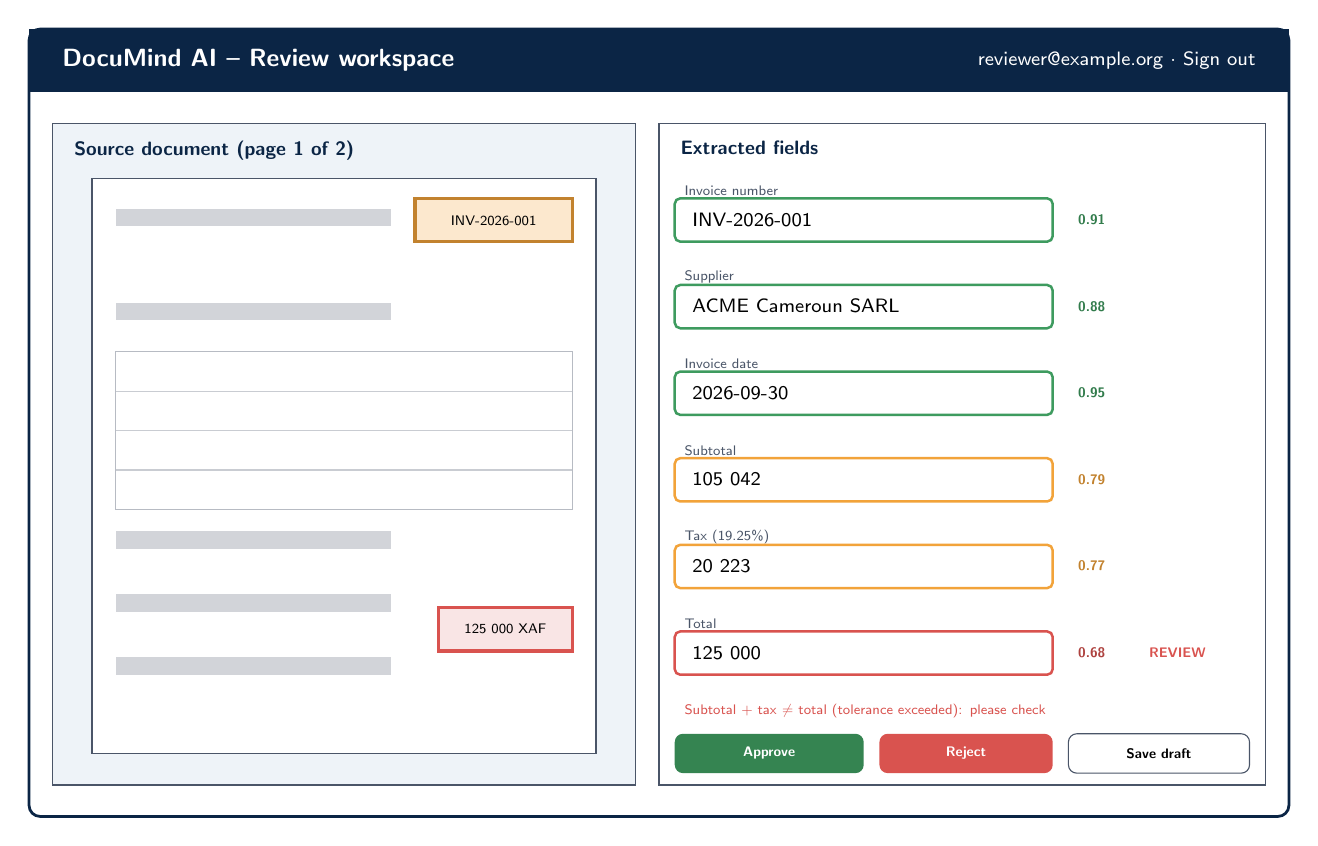
\begin{tikzpicture}[x=1cm,y=1cm]
\draw[rounded corners=4pt,fill=white,draw=navy,line width=1pt] (0,0) rectangle (16,10);
\fill[navy] (0,9.2) rectangle (16,10); \node[text=white,font=\sffamily\bfseries\small,anchor=west] at (0.3,9.6) {\projname{} -- Review workspace};
\node[text=white,font=\sffamily\scriptsize,anchor=east] at (15.7,9.6) {reviewer@example.org $\cdot$ Sign out};
\draw[fill=mist,draw=slate] (0.3,0.4) rectangle (7.7,8.8);
\node[font=\sffamily\scriptsize\bfseries,text=navy,anchor=north west] at (0.45,8.7) {Source document (page 1 of 2)};
\draw[fill=white,draw=slate] (0.8,0.8) rectangle (7.2,8.1);
\foreach \y in {7.5,6.3,3.4,2.6,1.8}{\fill[slate!25] (1.1,\y) rectangle (4.6,\y+0.22);}
\draw[amber!80!black,line width=1.2pt,fill=amber!25] (4.9,7.3) rectangle (6.9,7.85); \node[font=\sffamily\tiny] at (5.9,7.57) {INV-2026-001};
\draw[coral,line width=1.2pt,fill=coral!15] (5.2,2.1) rectangle (6.9,2.65); \node[font=\sffamily\tiny] at (6.05,2.38) {125 000 XAF};
\draw[slate!40] (1.1,5.9) rectangle (6.9,3.9); \foreach \y in {5.4,4.9,4.4}{\draw[slate!30] (1.1,\y) -- (6.9,\y);}
\draw[fill=white,draw=slate] (8.0,0.4) rectangle (15.7,8.8);
\node[font=\sffamily\scriptsize\bfseries,text=navy,anchor=north west] at (8.15,8.7) {Extracted fields};
\foreach \y/\n/\v/\cf/\col in {7.6/Invoice number/INV-2026-001/0.91/leaf, 6.5/Supplier/ACME Cameroun SARL/0.88/leaf, 5.4/Invoice date/2026-09-30/0.95/leaf, 4.3/Subtotal/105 042/0.79/amber, 3.2/Tax (19.25\%)/20 223/0.77/amber, 2.1/Total/125 000/0.68/coral}{
  \node[font=\sffamily\tiny,text=slate,anchor=west] at (8.2,\y+0.35) {\n};
  \draw[rounded corners=2pt,fill=white,draw=\col,line width=0.9pt] (8.2,\y-0.3) rectangle (13.0,\y+0.25);
  \node[font=\sffamily\scriptsize,anchor=west] at (8.3,\y-0.02) {\v};
  \node[font=\sffamily\tiny\bfseries,text=\col!80!black,anchor=west] at (13.2,\y-0.02) {\cf};}
\node[font=\sffamily\tiny\bfseries,text=coral,anchor=west] at (14.1,2.08) {REVIEW};
\node[font=\sffamily\tiny,text=coral,text width=6.8cm,anchor=north west] at (8.2,1.55) {Subtotal + tax $\neq$ total (tolerance exceeded): please check};
\draw[rounded corners=3pt,fill=leaf!85!black,draw=none] (8.2,0.55) rectangle (10.6,1.05); \node[text=white,font=\sffamily\bfseries\tiny] at (9.4,0.8) {Approve};
\draw[rounded corners=3pt,fill=coral,draw=none] (10.8,0.55) rectangle (13.0,1.05); \node[text=white,font=\sffamily\bfseries\tiny] at (11.9,0.8) {Reject};
\draw[rounded corners=3pt,fill=white,draw=slate] (13.2,0.55) rectangle (15.5,1.05); \node[font=\sffamily\bfseries\tiny] at (14.35,0.8) {Save draft};
\end{tikzpicture}
}
\caption{Wireframe of the review workspace (illustrative values from a synthetic invoice). Colour and a text label (REVIEW) are both used, so status never depends on colour alone.}\label{fig:wireframe}
\end{figure}

\section{Usability Guidelines}
Use clear status labels, not colour alone. Keep low-confidence values prominent but let users inspect the source evidence. Show why a field failed validation. Confirm before approval or rejection and prevent double-clicks from creating duplicate submissions. Provide loading, empty, success and error states. The Flutter app never contains database credentials or ERP secrets.

\chapter{Security, Privacy and Reliability}
\section{Security Controls}
\begin{itemize}
\item Enforce authentication and role-based authorisation in the backend, not only in the UI.
\item Hash passwords with a modern algorithm if local passwords are used.
\item Keep API keys, database passwords, signing keys and ERP credentials in environment-specific secret storage; commit only placeholders in \texttt{.env.example}.
\item Restrict extensions, MIME types, size and PDF page count; do not trust client-supplied MIME types alone.
\item Store files outside the public directory and serve them only after an authorisation check.
\item Use parameterised database access through the ORM and validate all input.
\item Apply rate limits and upload quotas when exposed beyond a trusted network.
\item Use HTTPS when deployed and restrict CORS to known origins.
\item Redact tokens, passwords and sensitive values from logs.
\item Back up the database and file store together and test restoration.
\end{itemize}

\section{Privacy and Governance}
Documents may contain personal, financial or confidential information. Define who may access them, why they are kept, for how long and how deletion works. Use synthetic or anonymised samples for demonstrations. Do not send documents to external OCR or AI services unless the data-handling implications and authorisation are understood.

\section{Reliability and Recovery}
Each processing step has a status and an error category. Retries are bounded and distinguish transient from permanent errors. Job state is persisted so a restart does not silently lose work. ERP submission is idempotent where possible. Database transactions protect related metadata changes, and file writes include cleanup or reconciliation for partial failures.

\chapter{Technology Stack and Rationale}
{\tblstart\small
\begin{longtable}{L{3.3cm}L{3.5cm}L{6.9cm}}
\hdrrow \hdr{Technology} & \hdr{Role} & \hdr{Rationale}\\ \endhead
Python 3.13 (recommended) & Backend and ML language & Widely used for APIs, image processing and training. Use a release supported by all dependencies; avoid pre-release interpreters.\\
FastAPI + Uvicorn & HTTP API and ASGI server & Type-aware validation and automatic OpenAPI documentation.\\
Pydantic & Schemas and settings & Validated, consistent data contracts.\\
SQLAlchemy + Alembic & ORM and migrations & Organised database access and reproducible schema changes.\\
MySQL 8 & Relational database & Metadata, fields, workflow state, users and audit records.\\
OpenCV & Image preprocessing & Denoising, thresholding and geometric correction.\\
PyTorch & Custom OCR model & Training, evaluation and inference.\\
Tesseract & Baseline OCR & Established engine for a fair comparison.\\
Flutter Web & User interface & One reusable widget toolkit for the dashboard.\\
Docker / Compose & Packaging and local orchestration & Reproducible environments and multi-container tests.\\
RabbitMQ + worker (later) & Background jobs & Decouples slow OCR from API requests.\\
Kubernetes (later) & Orchestration & Deploy and scale after the containerised system is stable.\\
\hline
\end{longtable}}
\section{Dependency Installation Strategy}
Do not install every dependency at once. Start from a supported Python version and a small API environment, verify the health endpoint, then add database, upload, preprocessing, OCR and UI in separate milestones. Pin tested versions. If installation fails, diagnose the Python version and the \emph{first} real error before adding compilers or unrelated packages. (A real example from this project: installing the optional ``standard'' extras of FastAPI on a very new Python tried to compile PyYAML; installing \texttt{fastapi} and \texttt{uvicorn} without extras on Python 3.13 avoids that.)

\chapter{Testing and Evaluation Plan}
\section{Testing Levels}
{\tblstart\small
\begin{longtable}{L{3.0cm}L{5.8cm}L{5.0cm}}
\hdrrow \hdr{Level} & \hdr{Examples} & \hdr{Evidence}\\ \endhead
Unit & File validation, normalisation, date/amount parsing, arithmetic rules, confidence policy. & Automated report with expected vs actual.\\
API & Authentication, upload, list, result, approval, forbidden access. & Status codes and schema checks.\\
Database & Foreign keys, constraints, migrations, rollback. & Test database results.\\
OCR evaluation & CER/WER for custom model and baseline on the same test set. & Dataset description, versions, tables.\\
End-to-end & Upload, process, review, approve, submit to sandbox. & Traceable run with state transitions.\\
Security & Wrong-role access, unsafe files, oversized uploads, secret leakage. & Pass/fail checklist and findings.\\
Recovery & OCR failure, database interruption, retry, duplicate ERP response. & Consistent status; no duplicate records.\\
Usability & Reviewer completes correction and approval tasks. & Observations and improvements.\\
\hline
\end{longtable}}

\section{Evaluation Metrics}
\begin{itemize}
\item \textbf{OCR:} CER, WER and inference time per page.
\item \textbf{Extraction:} precision, recall and F1 per field with a clear matching rule.
\item \textbf{Validation:} true errors detected, false alarms and misses on labelled cases.
\item \textbf{Workflow:} share completed without correction, share sent to review, rejection rate, failures.
\item \textbf{System:} median and 95th-percentile time, API error rate, retry success, resource use under a stated workload.
\item \textbf{ERP:} valid payload rate, outcomes, duplicate-prevention tests.
\end{itemize}

\section{Experiment Design}
Create a test set with verified transcriptions and field values. Run the custom model and the baseline on exactly the same held-out examples. Report dataset size, language mix, document types, preprocessing, model versions and hardware. Do not tune thresholds on the test set. Report field-level metrics, not a single accuracy that hides weak fields, and discuss failure cases such as skewed scans, stamps, low resolution, unusual layouts and ambiguous date or number formats.

\section{Acceptance Criteria for the Prototype}
\begin{enumerate}
\item A permitted user uploads a supported invoice and receives a stable document ID.
\item The original is stored privately and a persistent state is shown.
\item A supported invoice passes preprocessing, OCR, extraction and validation.
\item A reviewer inspects the source, corrects a field and approves or rejects.
\item Only an approved record reaches the ERP adapter.
\item A sandbox or mock integration demonstrates success, failure and safe retry.
\item OCR and extraction results from a held-out set are reported with a baseline comparison.
\item Automated tests cover core rules and authorisation boundaries.
\item A new developer can follow the documented setup from a clean environment.
\end{enumerate}

\chapter{Implementation Roadmap}
The project follows 18 phases grouped in four stages. The key principle is to make \emph{one complete workflow} work first -- upload, preprocess, recognise, extract, validate, review, send to a test ERP -- and only then scale the architecture.

\begin{figure}[H]\centering
\resizebox{\textwidth}{!}{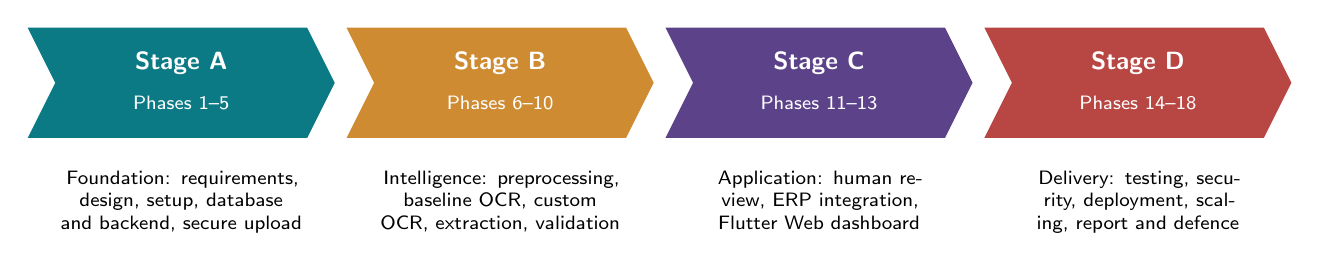
\begin{tikzpicture}[x=1cm,y=1cm]
\def\w{3.9}
\foreach \i/\c/\t/\p/\d in {%
  {0/teal/Stage A/Phases 1--5/Foundation: requirements, design, setup, database and backend, secure upload},%
  {1/amber/Stage B/Phases 6--10/Intelligence: preprocessing, baseline OCR, custom OCR, extraction, validation},%
  {2/violet/Stage C/Phases 11--13/Application: human review, ERP integration, Flutter Web dashboard},%
  {3/coral/Stage D/Phases 14--18/Delivery: testing, security, deployment, scaling, report and defence}}{
  \pgfmathsetmacro{\x}{\i*(\w+0.15)}
  \fill[\c!85!black] (\x,0) -- (\x+\w-0.35,0) -- (\x+\w,-0.7) -- (\x+\w-0.35,-1.4) -- (\x,-1.4) -- (\x+0.35,-0.7) -- cycle;
  \node[text=white,font=\sffamily\bfseries\small,align=center] at (\x+\w/2,-0.45) {\t};
  \node[text=white,font=\sffamily\scriptsize,align=center] at (\x+\w/2,-0.95) {\p};
  \node[font=\sffamily\scriptsize,text width=3.5cm,align=center,anchor=north] at (\x+\w/2,-1.7) {\d};}
\end{tikzpicture}
}
\caption{The four stages of the project.}\label{fig:stages}
\end{figure}

{\tblstart\footnotesize
\begin{longtable}{L{0.8cm}L{3.5cm}L{7.6cm}L{2.2cm}}
\hdrrow \hdr{No.} & \hdr{Phase} & \hdr{Main deliverable} & \hdr{Status}\\ \endhead
1 & Requirements and planning & Requirements specification (companion document) & \inprog\\
2 & System design and architecture & Architecture, UML, ER, API specification (this document) & \inprog\\
3 & Environment setup & Working development environment, repository & \inprog\\
4 & Database and backend foundation & Backend connected to MySQL, models, authentication & \inprog\\
5 & Document upload and storage & Secure upload, hashing, listing, retrieval & \todo\\
6 & Image preprocessing & Pipeline preparing pages for OCR & \todo\\
7 & Baseline OCR integration & OCR pipeline and baseline results & \todo\\
8 & Custom OCR model & Trained model with documented evaluation & \todo\\
9 & Information extraction & Structured invoice fields & \todo\\
10 & Validation and confidence & Accepted / rejected / review-required records & \todo\\
11 & Human review and correction & Review dashboard and correction workflow & \todo\\
12 & ERP integration & Adapter with mock or sandbox ERP & \todo\\
13 & Flutter Web dashboard & Functional web interface & \todo\\
14 & Testing and evaluation & Test reports and evaluation tables & \todo\\
15 & Security and reliability & Hardened, recoverable application & \todo\\
16 & Dockerisation and deployment & Deployed application & \todo\\
17 & Microservices and scalability & Modular deployment and scaling strategy & \todo\\
18 & Documentation and defence & Report, slides, demonstration & \todo\\
\hline
\end{longtable}}
\noindent Phases 1--4 are marked ``Partial'' because they are only partly complete; see Chapter~\ref{ch:status} for exact evidence.

\chapter{Deployment and Operations}\label{ch:deploy}
\section{Local Development}
Initially run the API locally and keep uploaded files in a private data directory excluded from Git. Keep credentials in a local \texttt{.env} that Git ignores; \texttt{.env.example} contains placeholders only. Use a separate development database and never experiment with destructive resets on important data.

\section{Docker Compose Stage}
\begin{figure}[H]\centering
\resizebox{\textwidth}{!}{\begin{tikzpicture}[x=1cm,y=1cm]
\node[box,fill=mist,minimum width=3.0cm] (br) at (1.6,6.3) {\textbf{Browser}\\\scriptsize Flutter Web};
\draw[rounded corners=6pt,fill=mint!60,draw=tealdark,line width=0.9pt] (3.7,-0.4) rectangle (14.9,8.1);
\node[font=\sffamily\bfseries\scriptsize,text=tealdark,anchor=north west] at (3.9,8.0) {Docker host (developer PC or VPS) -- network \texttt{idp-net}};
\node[boxT,text width=2.4cm,minimum height=1.5cm] (web) at (5.7,6.0) {\stereo{container}\\\textbf{web}\\\scriptsize nginx + Flutter build};
\node[boxA,text width=2.4cm,minimum height=1.5cm] (api) at (9.2,6.0) {\stereo{container}\\\textbf{backend}\\\scriptsize FastAPI :8000};
\node[boxA,text width=2.4cm,minimum height=1.5cm,dashed] (wrk) at (12.7,6.0) {\stereo{container}\\\textbf{worker}\\\scriptsize OCR jobs (later)};
\node[boxV,text width=2.4cm,minimum height=1.5cm] (db) at (9.2,2.8) {\stereo{container}\\\textbf{mysql}\\\scriptsize MySQL 8 :3306};
\node[boxV,text width=2.4cm,minimum height=1.5cm,dashed] (mq) at (12.7,2.8) {\stereo{container}\\\textbf{rabbitmq}\\\scriptsize broker (later)};
\node[box,fill=white,draw=slate,text width=2.4cm] (v2) at (5.7,2.8) {\stereo{volume}\\ \scriptsize file\_storage};
\node[box,fill=white,draw=slate,text width=2.4cm] (v1) at (9.2,0.4) {\stereo{volume}\\ \scriptsize mysql\_data};
\node[boxC,minimum width=2.4cm] (erp) at (17.3,6.0) {\textbf{ERP}\\\scriptsize Odoo or mock API};
\draw[arr] (br) -- node[lbl,above]{HTTPS} (web);
\draw[arr] (web) -- node[lbl,above]{/api} (api);
\draw[arr] (api) -- node[lbl,right]{SQL} (db);
\draw[arrd] (api.south east) -- (mq.north west);
\draw[arrd] (wrk.south) -- (mq.north);
\draw[arr] (db) -- (v1);
\draw[arr] (api.south west) -- (v2.north east);
\draw[arr] (api.north) -- ++(0,0.5) -| node[lbl,pos=0.25,above]{HTTPS API} (erp.north);
\end{tikzpicture}
}
\caption{Docker Compose deployment. Dashed boxes are later-stage components.}\label{fig:compose}
\end{figure}
Compose runs the API, MySQL and later the worker in separate containers on a private network with named volumes, health checks and non-root containers where practical. MySQL is not exposed to the internet and secrets are never baked into images.

\section{Kubernetes Stage}
\begin{figure}[H]\centering
\resizebox{\textwidth}{!}{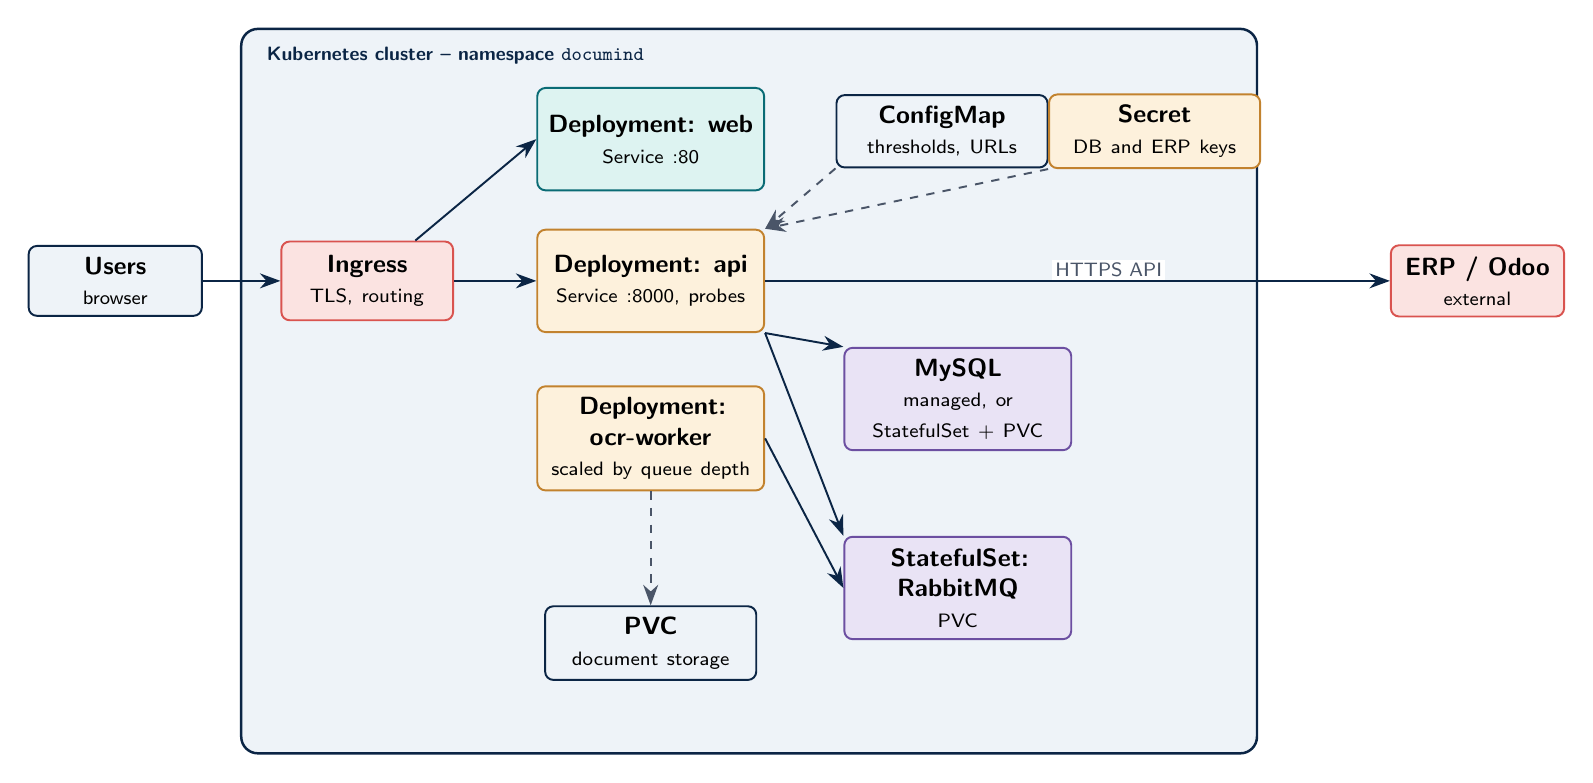
\begin{tikzpicture}[x=1cm,y=1cm]
\node[box,fill=mist,minimum width=2.2cm] (usr) at (1.1,5.4) {\textbf{Users}\\\scriptsize browser};
\draw[rounded corners=6pt,fill=mist,draw=navy,line width=0.9pt] (2.7,-0.6) rectangle (15.6,8.6);
\node[font=\sffamily\bfseries\scriptsize,text=navy,anchor=north west] at (2.9,8.5) {Kubernetes cluster -- namespace \texttt{documind}};
\node[boxC,text width=1.9cm,minimum height=1.0cm] (ing) at (4.3,5.4) {\textbf{Ingress}\\\scriptsize TLS, routing};
\node[boxT,text width=2.6cm,minimum height=1.3cm] (sw) at (7.9,7.2) {\textbf{Deployment: web}\\\scriptsize Service :80};
\node[boxA,text width=2.6cm,minimum height=1.3cm] (sa) at (7.9,5.4) {\textbf{Deployment: api}\\\scriptsize Service :8000, probes};
\node[boxA,text width=2.6cm,minimum height=1.3cm] (sk) at (7.9,3.4) {\textbf{Deployment: ocr-worker}\\\scriptsize scaled by queue depth};
\node[boxV,text width=2.6cm,minimum height=1.3cm] (sd) at (11.8,3.9) {\textbf{MySQL}\\\scriptsize managed, or StatefulSet + PVC};
\node[boxV,text width=2.6cm,minimum height=1.3cm] (sq) at (11.8,1.5) {\textbf{StatefulSet: RabbitMQ}\\\scriptsize PVC};
\node[box,text width=2.4cm] (cm) at (11.6,7.3) {\textbf{ConfigMap}\\\scriptsize thresholds, URLs};
\node[box,text width=2.4cm,fill=sand,draw=amber!80!black] (sec) at (14.3,7.3) {\textbf{Secret}\\\scriptsize DB and ERP keys};
\node[box,text width=2.4cm] (pvc) at (7.9,0.8) {\textbf{PVC}\\\scriptsize document storage};
\node[boxC,minimum width=2.2cm] (erp) at (18.4,5.4) {\textbf{ERP / Odoo}\\\scriptsize external};
\draw[arr] (usr) -- (ing);
\draw[arr] (ing) -- (sw.west);
\draw[arr] (ing) -- (sa);
\draw[arr] (sa.south east) -- (sd.north west);
\draw[arr] (sa.south east) -- (sq.north west);
\draw[arr] (sk.east) -- (sq.west);
\draw[arrd] (sk.south) -- (pvc.north);
\draw[arr] (sa.east) -- node[lbl,above,pos=0.55]{HTTPS API} (erp.west);
\draw[arrd] (cm.south west) -- (sa.north east);
\draw[arrd] (sec.south west) -- (sa.north east);
\end{tikzpicture}
}
\caption{Target Kubernetes layout (later stage).}\label{fig:k8s}
\end{figure}
Kubernetes is attempted only after the Compose tests pass. Likely resources are Deployments, Services, ConfigMaps, Secrets, persistent volumes or object storage, readiness and liveness probes, resource limits and an Ingress with TLS. A stateful database may stay outside the cluster for a student demonstration. Secrets are never committed as plain text.

\section{Observability}
Use structured logs with correlation IDs (document ID, run ID). Monitor queue depth, processing duration, OCR failure categories, review backlog, ERP failure rate and database availability. Do not log full document contents by default. The health endpoint reports availability without exposing credentials.

\chapter{Implementation Status}\label{ch:status}
This chapter separates what exists from what is only designed, so that the report never overstates progress.

\section{Backend Foundation (Phase 3--4, partial)}
{\tblstart\small
\begin{longtable}{L{4.6cm}L{1.9cm}L{7.3cm}}
\hdrrow \hdr{Item} & \hdr{Status} & \hdr{Evidence / note}\\ \endhead
FastAPI application with settings from environment & \done & Package \texttt{idp-phase1.zip}, \texttt{backend/app}.\\
Liveness endpoint \texttt{/api/v1/health} & \done & Tested; server started and endpoint answered.\\
Readiness endpoint \texttt{/api/v1/health/db} & \done & Returns 503 when MySQL is unreachable (tested); a successful MySQL connection has \emph{not} been verified yet.\\
Automated tests & \done & 4 tests passed in the build environment (Python 3.13).\\
Dockerfile and Docker Compose with MySQL 8 & \inprog & Written but \emph{not} built or run yet; must be tested on the student's machine.\\
Run on the student's Windows machine & \todo & Pending; earlier install attempts failed on Python 3.15 -- use Python 3.13.\\
SQLAlchemy models and Alembic migrations & \todo & Next step (Phase 4).\\
Authentication and roles & \todo & Phase 4.\\
\hline
\end{longtable}}

\section{Not Yet Started}
Document upload, preprocessing, baseline OCR, \textbf{custom OCR model (no model has been trained)}, extraction, validation, review workflow, ERP adapter, Flutter dashboard, security hardening, Kubernetes. The OCR model requires a labelled dataset that does not exist yet; its training and evaluation are scheduled in Phase 8.

\chapter{Risks and Mitigation}
\begin{figure}[H]\centering
\resizebox{0.72\textwidth}{!}{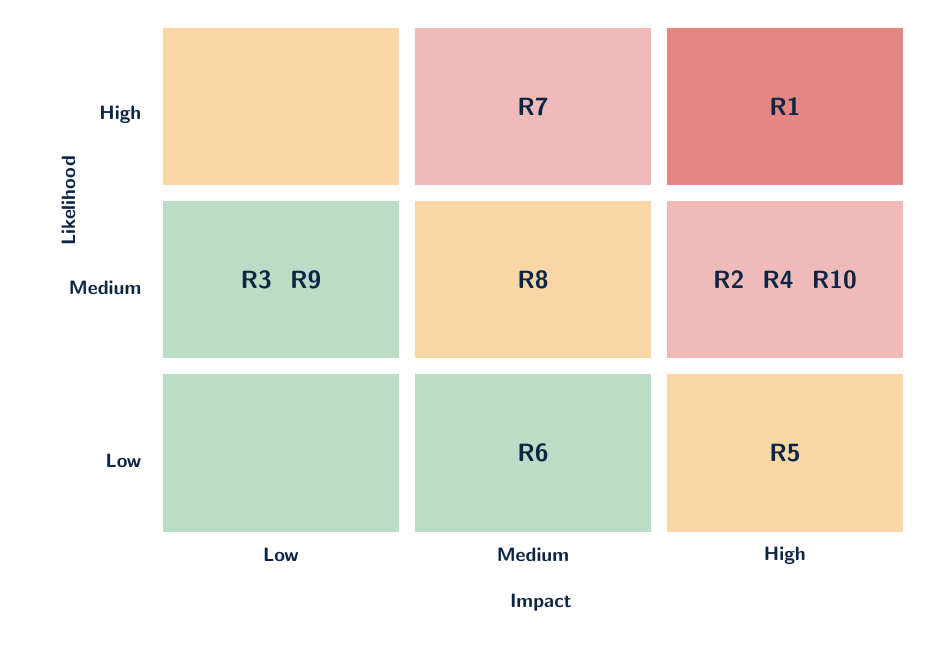
\begin{tikzpicture}[x=1cm,y=1cm]
\foreach \r/\ry in {0/High,1/Medium,2/Low}{
  \node[font=\sffamily\scriptsize\bfseries,text=navy,anchor=east] at (-0.15,{2.5-\r*2.2}) {\ry};}
\foreach \c/\cx in {0/Low,1/Medium,2/High}{
  \node[font=\sffamily\scriptsize\bfseries,text=navy] at ({1.5+\c*3.2},-3.1) {\cx};}
% cells (row 0 = high likelihood)
\foreach \r/\c/\col in {0/0/amber!45,0/1/coral!40,0/2/coral!70, 1/0/leaf!35,1/1/amber!45,1/2/coral!40, 2/0/leaf!35,2/1/leaf!35,2/2/amber!45}{
  \fill[\col] ({\c*3.2},{3.6-\r*2.2}) rectangle ({\c*3.2+3.0},{3.6-\r*2.2-2.0});}
\node[font=\sffamily\small\bfseries,text=navy] at (-1.6,2.5) {};
\node[rotate=90,font=\sffamily\scriptsize\bfseries,text=navy] at (-1.2,1.4) {Likelihood};
\node[font=\sffamily\scriptsize\bfseries,text=navy] at (4.8,-3.7) {Impact};
\node[font=\sffamily\small\bfseries,text=navy,align=center] at (7.9,2.6) {R1};  % high L, high I
\node[font=\sffamily\small\bfseries,text=navy,align=center] at (4.7,2.6) {R7};  % high L, medium I
\node[font=\sffamily\small\bfseries,text=navy,align=center] at (7.9,0.4) {R2 \ R4 \ R10}; % medium L, high I
\node[font=\sffamily\small\bfseries,text=navy,align=center] at (4.7,0.4) {R8};  % medium L, medium I
\node[font=\sffamily\small\bfseries,text=navy,align=center] at (1.5,0.4) {R3 \ R9}; % medium L, low I
\node[font=\sffamily\small\bfseries,text=navy,align=center] at (7.9,-1.8) {R5};  % low L, high I
\node[font=\sffamily\small\bfseries,text=navy,align=center] at (4.7,-1.8) {R6};  % low L, medium I
\end{tikzpicture}
}
\caption{Risk matrix (likelihood against impact). Identifiers refer to the table below; ratings are initial judgements to be revisited each phase.}\label{fig:risk}
\end{figure}
{\tblstart\small
\begin{longtable}{L{0.9cm}L{3.3cm}L{3.6cm}L{5.8cm}}
\hdrrow \hdr{ID} & \hdr{Risk} & \hdr{Impact} & \hdr{Mitigation}\\ \endhead
R1 & Insufficient labelled data & Custom OCR cannot be evaluated reliably. & Limit to invoices, create synthetic and carefully labelled data, document limitations, compare with a baseline.\\
R2 & Custom OCR under-performs & Low field quality, much manual review. & Baseline comparison, error analysis, better data and preprocessing, replaceable OCR interface.\\
R3 & Python/package incompatibility & Installation and development delays. & Python 3.13, pinned versions, incremental installs.\\
R4 & Unclear ERP API or no Odoo access & Integration cannot be completed early. & Generic adapter interface, mock/sandbox, gather ERP requirements early.\\
R5 & Sensitive documents exposed & Privacy and reputational harm. & Synthetic data, private storage, authorisation, minimal logs, retention rules.\\
R6 & Duplicate ERP records & Incorrect business data. & Idempotency keys, stored attempts, retry tests.\\
R7 & Scope grows too large & Core workflow unfinished. & Invoices only, limited field set, one baseline, one custom experiment, mock ERP.\\
R8 & Microservice overhead & More configuration and distributed failures. & Modular monolith first; split later.\\
R9 & OCR jobs crash & Documents get stuck. & Persisted status, bounded retries, manual retry.\\
R10 & Training hardware or time insufficient & Model cannot be trained or tuned. & Small model, cloud notebook or GPU access, reduce dataset scope.\\
\hline
\end{longtable}}

\chapter{Conclusion}
\projname{} proposes a complete workflow that turns incoming invoices into reviewed, validated, ERP-ready records. Its value depends on more than OCR: reliable file handling, extraction, validation, human review, secure storage, audit history and careful integration behaviour all matter. A custom OCR model is a meaningful research component only if it is trained on an appropriate dataset and compared fairly with a baseline.

The recommended order is incremental: API and database, secure upload, preprocessing and baseline OCR, custom OCR and extraction, review interface and ERP adapter. Containerisation, services, queues and Kubernetes come when the simpler system works and the added complexity is justified. Before submission, complete the supervisor details, choose the ERP or sandbox, add dataset documentation and measured results, and distinguish finished features from planned ones.

\appendix
\chapter{Glossary}
{\tblstart\small
\begin{longtable}{L{3.3cm}L{10.5cm}}
\hdrrow \hdr{Term} & \hdr{Meaning}\\ \endhead
API & Application Programming Interface: a defined way for software components to communicate.\\
CER / WER & Character / word error rate: edit errors divided by reference length.\\
CRNN & Convolutional recurrent neural network used for text recognition.\\
CTC & Connectionist Temporal Classification: loss and decoding for sequence recognition without explicit alignment.\\
ERP & Enterprise Resource Planning system.\\
Human-in-the-loop & Workflow in which a person reviews or corrects uncertain automated results.\\
IDP & Intelligent Document Processing: capture, recognise, extract, validate and route document information.\\
Idempotency & Property that makes repeated identical requests produce no duplicate effect.\\
OCR & Optical Character Recognition.\\
RBAC & Role-Based Access Control.\\
UML & Unified Modeling Language.\\
\hline
\end{longtable}}

\chapter{Suggested Demonstration Script}
\begin{enumerate}
\item Sign in as a document operator.
\item Upload a synthetic invoice; show its document ID and queued status.
\item Show the processing result and extracted fields.
\item Open a low-confidence field and compare it with the source.
\item Correct the field and enter a review note.
\item Approve the record and show the audit event.
\item Submit the approved record to the sandbox ERP adapter; show the external reference.
\item Submit again and show duplicate prevention.
\item Show the evaluation summary: custom OCR vs.\ baseline.
\end{enumerate}

\chapter{References and Further Reading}
Consult the official documentation and record exact versions and access dates in the final report.
\begin{itemize}
\item FastAPI: \url{https://fastapi.tiangolo.com/}
\item Flutter: \url{https://docs.flutter.dev/}
\item MySQL: \url{https://dev.mysql.com/doc/}
\item OpenCV: \url{https://docs.opencv.org/}
\item PyTorch: \url{https://pytorch.org/docs/}
\item Docker: \url{https://docs.docker.com/}
\item Kubernetes: \url{https://kubernetes.io/docs/}
\item SQLAlchemy: \url{https://docs.sqlalchemy.org/}
\item Alembic: \url{https://alembic.sqlalchemy.org/}
\end{itemize}

\begin{warnbox}[Before submission]
Complete the supervisor name, confirm your institution's formatting rules, verify each diagram against the final design, and replace planned or illustrative statements with implementation evidence.
\end{warnbox}


\end{document}
